\pdfoutput=1
%% Author: PGL  Porta Mana
%% Created: 2018-11-11T20:53:34+0200
%% Last-Updated: 2019-08-27T13:34:49+0200
%%%%%%%%%%%%%%%%%%%%%%%%%%%%%%%%%%%%%%%%%%%%%%%%%%%%%%%%%%%%%%%%%%%%%%%%%%%%
\newif\ifarxiv
\arxivfalse
\ifarxiv\pdfmapfile{+classico.map}\fi
\newif\ifafour
\afourfalse% true = A4, false = A5
\newif\iftypodisclaim % typographical disclaim on the side
\typodisclaimtrue
\newcommand*{\memfontfamily}{zplx}
\newcommand*{\memfontpack}{newpxtext}
\documentclass[\ifafour a4paper,12pt,\else a5paper,10pt,\fi%extrafontsizes,%
onecolumn,oneside,article,%french,italian,german,swedish,latin,
british%
]{memoir}
\newcommand*{\firstdraft}{11 November 2018}
\newcommand*{\firstpublished}{\firstdraft}
\newcommand*{\updated}{\ifarxiv***\else\today\fi}
\newcommand*{\propertitle}{Statistical relations between \textsc{snp}s and
  insomnia:\\ a simplified Bayesian study {\color{myred}\large[draft]}%
}% title uses LARGE; set Large for smaller
\newcommand*{\pdftitle}{Statistical relations between SNPs and insomnia: a simplified Bayesian study [draft]}
\newcommand*{\headtitle}{Bayesian study of \textsc{snp}s and insomnia}
\newcommand*{\pdfauthor}{D. Bragantini, P.G.L.  Porta Mana, I. C. G\"uzey, Y. Roudi}
\newcommand*{\headauthor}{Bragantini, Porta Mana, G\"uzey, Roudi}
\newcommand*{\reporthead}{\ifarxiv\else Open Science Framework \href{https://doi.org/10.31219/osf.io/***}{\textsc{doi}:10.31219/osf.io/***}\fi}% Report number

%%%%%%%%%%%%%%%%%%%%%%%%%%%%%%%%%%%%%%%%%%%%%%%%%%%%%%%%%%%%%%%%%%%%%%%%%%%%
%%% Calls to packages (uncomment as needed)
%%%%%%%%%%%%%%%%%%%%%%%%%%%%%%%%%%%%%%%%%%%%%%%%%%%%%%%%%%%%%%%%%%%%%%%%%%%%

%\usepackage{pifont}

%\usepackage{fontawesome}

\usepackage[T1]{fontenc} 
\input{glyphtounicode} \pdfgentounicode=1

\usepackage[utf8]{inputenx}

%\usepackage{newunicodechar}
% \newunicodechar{Ĕ}{\u{E}}
% \newunicodechar{ĕ}{\u{e}}
% \newunicodechar{Ĭ}{\u{I}}
% \newunicodechar{ĭ}{\u{\i}}
% \newunicodechar{Ŏ}{\u{O}}
% \newunicodechar{ŏ}{\u{o}}
% \newunicodechar{Ŭ}{\u{U}}
% \newunicodechar{ŭ}{\u{u}}
% \newunicodechar{Ā}{\=A}
% \newunicodechar{ā}{\=a}
% \newunicodechar{Ē}{\=E}
% \newunicodechar{ē}{\=e}
% \newunicodechar{Ī}{\=I}
% \newunicodechar{ī}{\={\i}}
% \newunicodechar{Ō}{\=O}
% \newunicodechar{ō}{\=o}
% \newunicodechar{Ū}{\=U}
% \newunicodechar{ū}{\=u}
% \newunicodechar{Ȳ}{\=Y}
% \newunicodechar{ȳ}{\=y}

\newcommand*{\bmmax}{0} % reduce number of bold fonts, before font packages
\newcommand*{\hmmax}{0} % reduce number of heavy fonts, before font packages

\usepackage{textcomp}

%\usepackage[normalem]{ulem}% package for underlining
% \makeatletter
% \def\ssout{\bgroup \ULdepth=-.35ex%\UL@setULdepth
%  \markoverwith{\lower\ULdepth\hbox
%    {\kern-.03em\vbox{\hrule width.2em\kern1.2\p@\hrule}\kern-.03em}}%
%  \ULon}
% \makeatother

\usepackage{amsmath}

\usepackage{mathtools}
\addtolength{\jot}{\jot} % increase spacing in multiline formulae
\setlength{\multlinegap}{0pt}

%\usepackage{empheq}% automatically calls amsmath and mathtools
%\newcommand*{\widefbox}[1]{\fbox{\hspace{1em}#1\hspace{1em}}}

%%%% empheq above seems more versatile than these:
%\usepackage{fancybox}
%\usepackage{framed}

% \usepackage[misc]{ifsym} % for dice
% \newcommand*{\diceone}{{\scriptsize\Cube{1}}}

\usepackage{amssymb}

\usepackage{amsxtra}

\usepackage[main=british,french,italian,german,swedish,latin,esperanto]{babel}\selectlanguage{british}
\newcommand*{\langfrench}{\foreignlanguage{french}}
\newcommand*{\langgerman}{\foreignlanguage{german}}
\newcommand*{\langitalian}{\foreignlanguage{italian}}
\newcommand*{\langswedish}{\foreignlanguage{swedish}}
\newcommand*{\langlatin}{\foreignlanguage{latin}}
\newcommand*{\langnohyph}{\foreignlanguage{nohyphenation}}

\usepackage[autostyle=false,autopunct=false,english=british]{csquotes}
\setquotestyle{british}

\usepackage{amsthm}
\newcommand*{\QED}{\textsc{q.e.d.}}
\renewcommand*{\qedsymbol}{\QED}
\theoremstyle{remark}
\newtheorem{note}{Note}
\newtheorem*{remark}{Note}
\newtheoremstyle{innote}{\parsep}{\parsep}{\footnotesize}{}{}{}{0pt}{}
\theoremstyle{innote}
\newtheorem*{innote}{}

\usepackage[shortlabels,inline]{enumitem}
\SetEnumitemKey{para}{itemindent=\parindent,leftmargin=0pt,listparindent=\parindent,parsep=0pt,itemsep=\topsep}
% \begin{asparaenum} = \begin{enumerate}[para]
% \begin{inparaenum} = \begin{enumerate*}
\setlist[enumerate,2]{label=\alph*.}
\setlist[enumerate]{label=\arabic*.,leftmargin=1.5\parindent}
\setlist[itemize]{leftmargin=1.5\parindent}
\setlist[description]{leftmargin=1.5\parindent}
% old alternative:
% \setlist[enumerate,2]{label=\alph*.}
% \setlist[enumerate]{leftmargin=\parindent}
% \setlist[itemize]{leftmargin=\parindent}
% \setlist[description]{leftmargin=\parindent}

\usepackage[babel,theoremfont,largesc]{newpxtext}

\usepackage[bigdelims,nosymbolsc%,smallerops % probably arXiv doesn't have it
]{newpxmath}
\linespread{1.083}%\useosf
%% smaller operators for old version of newpxmath
\makeatletter
\def\re@DeclareMathSymbol#1#2#3#4{%
    \let#1=\undefined
    \DeclareMathSymbol{#1}{#2}{#3}{#4}}
%\re@DeclareMathSymbol{\bigsqcupop}{\mathop}{largesymbols}{"46}
%\re@DeclareMathSymbol{\bigodotop}{\mathop}{largesymbols}{"4A}
\re@DeclareMathSymbol{\bigoplusop}{\mathop}{largesymbols}{"4C}
\re@DeclareMathSymbol{\bigotimesop}{\mathop}{largesymbols}{"4E}
\re@DeclareMathSymbol{\sumop}{\mathop}{largesymbols}{"50}
\re@DeclareMathSymbol{\prodop}{\mathop}{largesymbols}{"51}
\re@DeclareMathSymbol{\bigcupop}{\mathop}{largesymbols}{"53}
\re@DeclareMathSymbol{\bigcapop}{\mathop}{largesymbols}{"54}
%\re@DeclareMathSymbol{\biguplusop}{\mathop}{largesymbols}{"55}
\re@DeclareMathSymbol{\bigwedgeop}{\mathop}{largesymbols}{"56}
\re@DeclareMathSymbol{\bigveeop}{\mathop}{largesymbols}{"57}
%\re@DeclareMathSymbol{\bigcupdotop}{\mathop}{largesymbols}{"DF}
%\re@DeclareMathSymbol{\bigcapplusop}{\mathop}{largesymbolsPXA}{"00}
%\re@DeclareMathSymbol{\bigsqcupplusop}{\mathop}{largesymbolsPXA}{"02}
%\re@DeclareMathSymbol{\bigsqcapplusop}{\mathop}{largesymbolsPXA}{"04}
%\re@DeclareMathSymbol{\bigsqcapop}{\mathop}{largesymbolsPXA}{"06}
\re@DeclareMathSymbol{\bigtimesop}{\mathop}{largesymbolsPXA}{"10}
%\re@DeclareMathSymbol{\coprodop}{\mathop}{largesymbols}{"60}
%\re@DeclareMathSymbol{\varprod}{\mathop}{largesymbolsPXA}{16}
\makeatother
%%
%% With euler font cursive for Greek letters - the [1] means 100% scaling
\DeclareFontFamily{U}{egreek}{\skewchar\font'177}%
\DeclareFontShape{U}{egreek}{m}{n}{<-6>s*[1]eurm5 <6-8>s*[1]eurm7 <8->s*[1]eurm10}{}%
\DeclareFontShape{U}{egreek}{m}{it}{<->s*[1]eurmo10}{}%
\DeclareFontShape{U}{egreek}{b}{n}{<-6>s*[1]eurb5 <6-8>s*[1]eurb7 <8->s*[1]eurb10}{}%
\DeclareFontShape{U}{egreek}{b}{it}{<->s*[1]eurbo10}{}%
\DeclareSymbolFont{egreeki}{U}{egreek}{m}{it}%
\SetSymbolFont{egreeki}{bold}{U}{egreek}{b}{it}% from the amsfonts package
\DeclareSymbolFont{egreekr}{U}{egreek}{m}{n}%
\SetSymbolFont{egreekr}{bold}{U}{egreek}{b}{n}% from the amsfonts package
% Take also \sum, \prod, \coprod symbols from Euler fonts
\DeclareFontFamily{U}{egreekx}{\skewchar\font'177}
\DeclareFontShape{U}{egreekx}{m}{n}{%
       <-7.5>s*[0.9]euex7%
    <7.5-8.5>s*[0.9]euex8%
    <8.5-9.5>s*[0.9]euex9%
    <9.5->s*[0.9]euex10%
}{}
\DeclareSymbolFont{egreekx}{U}{egreekx}{m}{n}
\DeclareMathSymbol{\sumop}{\mathop}{egreekx}{"50}
\DeclareMathSymbol{\prodop}{\mathop}{egreekx}{"51}
\DeclareMathSymbol{\coprodop}{\mathop}{egreekx}{"60}
\makeatletter
\def\sum{\DOTSI\sumop\slimits@}
\def\prod{\DOTSI\prodop\slimits@}
\def\coprod{\DOTSI\coprodop\slimits@}
\makeatother
% Greek letters not usually given in LaTeX.
\DeclareMathSymbol{\varpartial}{\mathalpha}{egreeki}{"40}
\DeclareMathSymbol{\partialup}{\mathalpha}{egreekr}{"40}
\DeclareMathSymbol{\alpha}{\mathalpha}{egreeki}{"0B}
\DeclareMathSymbol{\beta}{\mathalpha}{egreeki}{"0C}
\DeclareMathSymbol{\gamma}{\mathalpha}{egreeki}{"0D}
\DeclareMathSymbol{\delta}{\mathalpha}{egreeki}{"0E}
\DeclareMathSymbol{\epsilon}{\mathalpha}{egreeki}{"0F}
\DeclareMathSymbol{\zeta}{\mathalpha}{egreeki}{"10}
\DeclareMathSymbol{\eta}{\mathalpha}{egreeki}{"11}
\DeclareMathSymbol{\theta}{\mathalpha}{egreeki}{"12}
\DeclareMathSymbol{\iota}{\mathalpha}{egreeki}{"13}
\DeclareMathSymbol{\kappa}{\mathalpha}{egreeki}{"14}
\DeclareMathSymbol{\lambda}{\mathalpha}{egreeki}{"15}
\DeclareMathSymbol{\mu}{\mathalpha}{egreeki}{"16}
\DeclareMathSymbol{\nu}{\mathalpha}{egreeki}{"17}
\DeclareMathSymbol{\xi}{\mathalpha}{egreeki}{"18}
\DeclareMathSymbol{\omicron}{\mathalpha}{egreeki}{"6F}
\DeclareMathSymbol{\pi}{\mathalpha}{egreeki}{"19}
\DeclareMathSymbol{\rho}{\mathalpha}{egreeki}{"1A}
\DeclareMathSymbol{\sigma}{\mathalpha}{egreeki}{"1B}
 \DeclareMathSymbol{\tau}{\mathalpha}{egreeki}{"1C}
\DeclareMathSymbol{\upsilon}{\mathalpha}{egreeki}{"1D}
\DeclareMathSymbol{\phi}{\mathalpha}{egreeki}{"1E}
\DeclareMathSymbol{\chi}{\mathalpha}{egreeki}{"1F}
\DeclareMathSymbol{\psi}{\mathalpha}{egreeki}{"20}
\DeclareMathSymbol{\omega}{\mathalpha}{egreeki}{"21}
\DeclareMathSymbol{\varepsilon}{\mathalpha}{egreeki}{"22}
\DeclareMathSymbol{\vartheta}{\mathalpha}{egreeki}{"23}
\DeclareMathSymbol{\varpi}{\mathalpha}{egreeki}{"24}
\let\varrho\rho 
\let\varsigma\sigma
 \let\varkappa\kappa
\DeclareMathSymbol{\varphi}{\mathalpha}{egreeki}{"27}
%
\DeclareMathSymbol{\varAlpha}{\mathalpha}{egreeki}{"41}
\DeclareMathSymbol{\varBeta}{\mathalpha}{egreeki}{"42}
\DeclareMathSymbol{\varGamma}{\mathalpha}{egreeki}{"00}
\DeclareMathSymbol{\varDelta}{\mathalpha}{egreeki}{"01}
\DeclareMathSymbol{\varEpsilon}{\mathalpha}{egreeki}{"45}
\DeclareMathSymbol{\varZeta}{\mathalpha}{egreeki}{"5A}
\DeclareMathSymbol{\varEta}{\mathalpha}{egreeki}{"48}
\DeclareMathSymbol{\varTheta}{\mathalpha}{egreeki}{"02}
 \DeclareMathSymbol{\varIota}{\mathalpha}{egreeki}{"49}
\DeclareMathSymbol{\varKappa}{\mathalpha}{egreeki}{"4B}
\DeclareMathSymbol{\varLambda}{\mathalpha}{egreeki}{"03}
\DeclareMathSymbol{\varMu}{\mathalpha}{egreeki}{"4D}
\DeclareMathSymbol{\varNu}{\mathalpha}{egreeki}{"4E}
\DeclareMathSymbol{\varXi}{\mathalpha}{egreeki}{"04}
\DeclareMathSymbol{\varOmicron}{\mathalpha}{egreeki}{"4F}
\DeclareMathSymbol{\varPi}{\mathalpha}{egreeki}{"05}
\DeclareMathSymbol{\varRho}{\mathalpha}{egreeki}{"50}
\DeclareMathSymbol{\varSigma}{\mathalpha}{egreeki}{"06}
\DeclareMathSymbol{\varTau}{\mathalpha}{egreeki}{"54}
\DeclareMathSymbol{\varUpsilon}{\mathalpha}{egreeki}{"07}
\DeclareMathSymbol{\varPhi}{\mathalpha}{egreeki}{"08}
\DeclareMathSymbol{\varChi}{\mathalpha}{egreeki}{"58}
\DeclareMathSymbol{\varPsi}{\mathalpha}{egreeki}{"09}
\DeclareMathSymbol{\varOmega}{\mathalpha}{egreeki}{"0A} 
%
\DeclareMathSymbol{\Alpha}{\mathalpha}{egreekr}{"41}
\DeclareMathSymbol{\Beta}{\mathalpha}{egreekr}{"42}
\DeclareMathSymbol{\Gamma}{\mathalpha}{egreekr}{"00}
\DeclareMathSymbol{\Delta}{\mathalpha}{egreekr}{"01}
\DeclareMathSymbol{\Epsilon}{\mathalpha}{egreekr}{"45}
\DeclareMathSymbol{\Zeta}{\mathalpha}{egreekr}{"5A}
\DeclareMathSymbol{\Eta}{\mathalpha}{egreekr}{"48}
\DeclareMathSymbol{\Theta}{\mathalpha}{egreekr}{"02}
\DeclareMathSymbol{\Iota}{\mathalpha}{egreekr}{"49}
\DeclareMathSymbol{\Kappa}{\mathalpha}{egreekr}{"4B}
\DeclareMathSymbol{\Lambda}{\mathalpha}{egreekr}{"03}
\DeclareMathSymbol{\Mu}{\mathalpha}{egreekr}{"4D}
\DeclareMathSymbol{\Nu}{\mathalpha}{egreekr}{"4E}
\DeclareMathSymbol{\Xi}{\mathalpha}{egreekr}{"04}
\DeclareMathSymbol{\Omicron}{\mathalpha}{egreekr}{"4F}
\DeclareMathSymbol{\Pi}{\mathalpha}{egreekr}{"05}
\DeclareMathSymbol{\Rho}{\mathalpha}{egreekr}{"50}
\DeclareMathSymbol{\Sigma}{\mathalpha}{egreekr}{"06}
\DeclareMathSymbol{\Tau}{\mathalpha}{egreekr}{"54}
\DeclareMathSymbol{\Upsilon}{\mathalpha}{egreekr}{"07}
\DeclareMathSymbol{\Phi}{\mathalpha}{egreekr}{"08}
\DeclareMathSymbol{\Chi}{\mathalpha}{egreekr}{"58}
\DeclareMathSymbol{\Psi}{\mathalpha}{egreekr}{"09}
\DeclareMathSymbol{\Omega}{\mathalpha}{egreekr}{"0A}
%
\DeclareMathSymbol{\alphaup}{\mathalpha}{egreekr}{"0B}
\DeclareMathSymbol{\betaup}{\mathalpha}{egreekr}{"0C}
\DeclareMathSymbol{\gammaup}{\mathalpha}{egreekr}{"0D}
 \DeclareMathSymbol{\deltaup}{\mathalpha}{egreekr}{"0E}
\DeclareMathSymbol{\epsilonup}{\mathalpha}{egreekr}{"0F}
\DeclareMathSymbol{\zetaup}{\mathalpha}{egreekr}{"10}
\DeclareMathSymbol{\etaup}{\mathalpha}{egreekr}{"11}
\DeclareMathSymbol{\thetaup}{\mathalpha}{egreekr}{"12}
\DeclareMathSymbol{\iotaup}{\mathalpha}{egreekr}{"13}
\DeclareMathSymbol{\kappaup}{\mathalpha}{egreekr}{"14}
\DeclareMathSymbol{\lambdaup}{\mathalpha}{egreekr}{"15}
\DeclareMathSymbol{\muup}{\mathalpha}{egreekr}{"16}
\DeclareMathSymbol{\nuup}{\mathalpha}{egreekr}{"17}
\DeclareMathSymbol{\xiup}{\mathalpha}{egreekr}{"18}
\DeclareMathSymbol{\omicronup}{\mathalpha}{egreekr}{"6F}
  \DeclareMathSymbol{\piup}{\mathalpha}{egreekr}{"19}
\DeclareMathSymbol{\rhoup}{\mathalpha}{egreekr}{"1A}
\DeclareMathSymbol{\sigmaup}{\mathalpha}{egreekr}{"1B}
\DeclareMathSymbol{\tauup}{\mathalpha}{egreekr}{"1C}
\DeclareMathSymbol{\upsilonup}{\mathalpha}{egreekr}{"1D}
\DeclareMathSymbol{\phiup}{\mathalpha}{egreekr}{"1E}
\DeclareMathSymbol{\chiup}{\mathalpha}{egreekr}{"1F}
\DeclareMathSymbol{\psiup}{\mathalpha}{egreekr}{"20}
\DeclareMathSymbol{\omegaup}{\mathalpha}{egreekr}{"21}
\DeclareMathSymbol{\varepsilonup}{\mathalpha}{egreekr}{"22}
\DeclareMathSymbol{\varthetaup}{\mathalpha}{egreekr}{"23}
\DeclareMathSymbol{\varpiup}{\mathalpha}{egreekr}{"24}
\let\varrhoup\rhoup 
\let\varsigmaup\sigmaup
\let\varkappaup\kappaup
\DeclareMathSymbol{\varphiup}{\mathalpha}{egreekr}{"27}
% Greek letters not usually given in LaTeX.

%\usepackage%[scaled=0.9]%
%{classico}%  Optima as sans-serif font
\renewcommand\sfdefault{uop}
\DeclareMathAlphabet{\mathsf}  {T1}{\sfdefault}{m}{sl}
\SetMathAlphabet{\mathsf}{bold}{T1}{\sfdefault}{b}{sl}
%\newcommand*{\mathte}[1]{\textbf{\textit{\textsf{#1}}}}
% Upright sans-serif math alphabet
% \DeclareMathAlphabet{\mathsu}  {T1}{\sfdefault}{m}{n}
% \SetMathAlphabet{\mathsu}{bold}{T1}{\sfdefault}{b}{n}

% DejaVu Mono as typewriter text
\usepackage[scaled=0.84]{DejaVuSansMono}

\usepackage{mathdots}

\usepackage[usenames]{xcolor}
% Tol (2012) colour-blind-, print-, screen-friendly colours, alternative scheme; Munsell terminology
\definecolor{mypurpleblue}{RGB}{68,119,170}
\definecolor{myblue}{RGB}{102,204,238}
\definecolor{mygreen}{RGB}{34,136,51}
\definecolor{myyellow}{RGB}{204,187,68}
\definecolor{myred}{RGB}{238,102,119}
\definecolor{myredpurple}{RGB}{170,51,119}
\definecolor{mygrey}{RGB}{187,187,187}
% Tol (2012) colour-blind-, print-, screen-friendly colours; Munsell terminology
% \definecolor{lbpurple}{RGB}{51,34,136}
% \definecolor{lblue}{RGB}{136,204,238}
% \definecolor{lbgreen}{RGB}{68,170,153}
% \definecolor{lgreen}{RGB}{17,119,51}
% \definecolor{lgyellow}{RGB}{153,153,51}
% \definecolor{lyellow}{RGB}{221,204,119}
% \definecolor{lred}{RGB}{204,102,119}
% \definecolor{lpred}{RGB}{136,34,85}
% \definecolor{lrpurple}{RGB}{170,68,153}
\definecolor{lgrey}{RGB}{221,221,221}
%\newcommand*\mycolourbox[1]{%
%\colorbox{mygrey}{\hspace{1em}#1\hspace{1em}}}
\colorlet{shadecolor}{lgrey}

\usepackage{bm}

\usepackage{microtype}

\usepackage[backend=biber,mcite,%subentry,
citestyle=authoryear-comp,bibstyle=pglpm-authoryear,autopunct=false,sorting=ny,sortcites=false,natbib=false,maxcitenames=1,maxbibnames=8,minbibnames=8,giveninits=true,uniquename=false,uniquelist=false,maxalphanames=1,block=space,hyperref=true,defernumbers=false,useprefix=true,sortupper=false,language=british,parentracker=false]{biblatex}
\DeclareSortingScheme{ny}{\sort{\field{sortname}\field{author}\field{editor}}\sort{\field{year}}}
\iffalse\makeatletter%%% replace parenthesis with brackets
\newrobustcmd*{\parentexttrack}[1]{%
  \begingroup
  \blx@blxinit
  \blx@setsfcodes
  \blx@bibopenparen#1\blx@bibcloseparen
  \endgroup}
\AtEveryCite{%
  \let\parentext=\parentexttrack%
  \let\bibopenparen=\bibopenbracket%
  \let\bibcloseparen=\bibclosebracket}
\makeatother\fi
\DefineBibliographyExtras{british}{\def\finalandcomma{\addcomma}}
\renewcommand*{\finalnamedelim}{\addcomma\space}
\setcounter{biburlnumpenalty}{1}
\setcounter{biburlucpenalty}{0}
\setcounter{biburllcpenalty}{1}
\DeclareDelimFormat{multicitedelim}{\addcomma\space}
\DeclareDelimFormat{compcitedelim}{\addcomma\space}
\DeclareDelimFormat{postnotedelim}{\space}
\ifarxiv\else\addbibresource{portamanabib.bib}\fi
\renewcommand{\bibfont}{\footnotesize}
%\appto{\citesetup}{\footnotesize}% smaller font for citations
\defbibheading{bibliography}[\bibname]{\section*{#1}\addcontentsline{toc}{section}{#1}%\markboth{#1}{#1}
}
\newcommand*{\citep}{\footcites}
\newcommand*{\citey}{\footcites}
%\renewcommand*{\cite}{\parencite}
%\renewcommand*{\cites}{\parencites}
\providecommand{\href}[2]{#2}
\providecommand{\eprint}[2]{\texttt{\href{#1}{#2}}}
\newcommand*{\amp}{\&}
% \newcommand*{\citein}[2][]{\textnormal{\textcite[#1]{#2}}%\addtocategory{extras}{#2}
% }
\newcommand*{\citein}[2][]{\textnormal{\textcite[#1]{#2}}%\addtocategory{extras}{#2}
}
\newcommand*{\citebi}[2][]{\textcite[#1]{#2}%\addtocategory{extras}{#2}
}
\newcommand*{\subtitleproc}[1]{}
\newcommand*{\chapb}{ch.}
%
% \def\arxivp{}
% \def\mparcp{}
% \def\philscip{}
% \def\biorxivp{}
% \newcommand*{\arxivsi}{\texttt{arXiv} eprints available at \url{http://arxiv.org/}.\\}
% \newcommand*{\mparcsi}{\texttt{mp\_arc} eprints available at \url{http://www.ma.utexas.edu/mp_arc/}.\\}
% \newcommand*{\philscisi}{\texttt{philsci} eprints available at \url{http://philsci-archive.pitt.edu/}.\\}
% \newcommand*{\biorxivsi}{\texttt{bioRxiv} eprints available at \url{http://biorxiv.org/}.\\}
\newcommand*{\arxiveprint}[1]{%\global\def\arxivp{\arxivsi}%\citeauthor{0arxivcite}\addtocategory{ifarchcit}{0arxivcite}%eprint
\texttt{\urlalt{https://arxiv.org/abs/#1}{arXiv:\hspace{0pt}#1}}%
%\texttt{\href{http://arxiv.org/abs/#1}{\protect\url{arXiv:#1}}}%
%\renewcommand{\arxivnote}{\texttt{arXiv} eprints available at \url{http://arxiv.org/}.}
}
\newcommand*{\haleprint}[1]{%\global\def\arxivp{\arxivsi}%\citeauthor{0arxivcite}\addtocategory{ifarchcit}{0arxivcite}%eprint
\texttt{\urlalt{https://hal.archives-ouvertes.fr/#1}{HAL:\hspace{0pt}#1}}%
%\texttt{\href{http://arxiv.org/abs/#1}{\protect\url{arXiv:#1}}}%
%\renewcommand{\arxivnote}{\texttt{arXiv} eprints available at \url{http://arxiv.org/}.}
}
\newcommand*{\mparceprint}[1]{%\global\def\mparcp{\mparcsi}%\citeauthor{0mparccite}\addtocategory{ifarchcit}{0mparccite}%eprint
\texttt{\urlalt{http://www.ma.utexas.edu/mp_arc-bin/mpa?yn=#1}{mp\_arc:\hspace{0pt}#1}}%
%\texttt{\href{http://www.ma.utexas.edu/mp_arc-bin/mpa?yn=#1}{\protect\url{mp_arc:#1}}}%
%\providecommand{\mparcnote}{\texttt{mp_arc} eprints available at \url{http://www.ma.utexas.edu/mp_arc/}.}
}
\newcommand*{\philscieprint}[1]{%\global\def\philscip{\philscisi}%\citeauthor{0philscicite}\addtocategory{ifarchcit}{0philscicite}%eprint
\texttt{\urlalt{http://philsci-archive.pitt.edu/archive/#1}{PhilSci:\hspace{0pt}#1}}%
%\texttt{\href{http://philsci-archive.pitt.edu/archive/#1}{\protect\url{PhilSci:#1}}}%
%\providecommand{\mparcnote}{\texttt{philsci} eprints available at \url{http://philsci-archive.pitt.edu/}.}
}
\newcommand*{\biorxiveprint}[1]{%\global\def\biorxivp{\biorxivsi}%\citeauthor{0arxivcite}\addtocategory{ifarchcit}{0arxivcite}%eprint
\texttt{\urlalt{https://doi.org/10.1101/#1}{bioRxiv doi:\hspace{0pt}10.1101/#1}}%
%\texttt{\href{http://arxiv.org/abs/#1}{\protect\url{arXiv:#1}}}%
%\renewcommand{\arxivnote}{\texttt{arXiv} eprints available at \url{http://arxiv.org/}.}
}
\newcommand*{\osfeprint}[1]{%
\texttt{\urlalt{https://doi.org/10.17605/osf.io/#1}{Open Science Framework doi:10.17605/osf.io/#1}}%
}

\usepackage{graphicx}

%\usepackage{wrapfig}

%\usepackage{tikz-cd}

\PassOptionsToPackage{hyphens}{url}\usepackage[hypertexnames=false]{hyperref}

\usepackage[depth=4]{bookmark}
\hypersetup{colorlinks=true,bookmarksnumbered,pdfborder={0 0 0.25},citebordercolor={0.2667 0.4667 0.6667},citecolor=mypurpleblue,linkbordercolor={0.6667 0.2 0.4667},linkcolor=myredpurple,urlbordercolor={0.1333 0.5333 0.2},urlcolor=mygreen,breaklinks=true,pdftitle={\pdftitle},pdfauthor={\pdfauthor}}
% \usepackage[vertfit=local]{breakurl}% only for arXiv
\providecommand*{\urlalt}{\href}

\usepackage[british]{datetime2}
\DTMnewdatestyle{mydate}%
{% definitions
\renewcommand*{\DTMdisplaydate}[4]{%
\number##3\ \DTMenglishmonthname{##2} ##1}%
\renewcommand*{\DTMDisplaydate}{\DTMdisplaydate}%
}
\DTMsetdatestyle{mydate}

%%%%%%%%%%%%%%%%%%%%%%%%%%%%%%%%%%%%%%%%%%%%%%%%%%%%%%%%%%%%%%%%%%%%%%%%%%%%
%%% Layout. I do not know on which kind of paper the reader will print the
%%% paper on (A4? letter? one-sided? double-sided?). So I choose A5, which
%%% provides a good layout for reading on screen and save paper if printed
%%% two pages per sheet. Average length line is 66 characters and page
%%% numbers are centred.
%%%%%%%%%%%%%%%%%%%%%%%%%%%%%%%%%%%%%%%%%%%%%%%%%%%%%%%%%%%%%%%%%%%%%%%%%%%%
\ifafour\setstocksize{297mm}{210mm}%{*}% A4
\else\setstocksize{210mm}{5.5in}%{*}% 210x139.7
\fi
\settrimmedsize{\stockheight}{\stockwidth}{*}
\setlxvchars[\normalfont] %313.3632pt for a 66-characters line
\setxlvchars[\normalfont]
\setlength{\trimtop}{0pt}
\setlength{\trimedge}{\stockwidth}
\addtolength{\trimedge}{-\paperwidth}
% The length of the normalsize alphabet is 133.05988pt - 10 pt = 26.1408pc
% The length of the normalsize alphabet is 159.6719pt - 12pt = 30.3586pc
% Bringhurst gives 32pc as boundary optimal with 69 ch per line
% The length of the normalsize alphabet is 191.60612pt - 14pt = 35.8634pc
\ifafour\settypeblocksize{*}{32pc}{1.618} % A4
%\setulmargins{*}{*}{1.667}%gives 5/3 margins % 2 or 1.667
\else\settypeblocksize{*}{26pc}{1.618}% nearer to a 66-line newpx and preserves GR
\fi
\setulmargins{*}{*}{1}%gives equal margins
\setlrmargins{*}{*}{*}
\setheadfoot{\onelineskip}{2.5\onelineskip}
\setheaderspaces{*}{2\onelineskip}{*}
\setmarginnotes{2ex}{10mm}{0pt}
\checkandfixthelayout[nearest]
\fixpdflayout
%%% End layout
%% this fixes missing white spaces
\pdfmapline{+dummy-space <dummy-space.pfb}\pdfinterwordspaceon%

%%% Sectioning
\newcommand*{\asudedication}[1]{%
{\par\centering\textit{#1}\par}}
\newenvironment{acknowledgements}{\section*{Thanks}\addcontentsline{toc}{section}{Thanks}}{\par}
\makeatletter\renewcommand{\appendix}{\par
  \bigskip{\centering
   \interlinepenalty \@M
   \normalfont
   \printchaptertitle{\sffamily\appendixpagename}\par}
  \setcounter{section}{0}%
  \gdef\@chapapp{\appendixname}%
  \gdef\thesection{\@Alph\c@section}%
  \anappendixtrue}\makeatother
\counterwithout{section}{chapter}
\setsecnumformat{\upshape\csname the#1\endcsname\quad}
\setsecheadstyle{\large\bfseries\sffamily%
\centering}
\setsubsecheadstyle{\bfseries\sffamily%
\raggedright}
%\setbeforesecskip{-1.5ex plus 1ex minus .2ex}% plus 1ex minus .2ex}
%\setaftersecskip{1.3ex plus .2ex }% plus 1ex minus .2ex}
%\setsubsubsecheadstyle{\bfseries\sffamily\slshape\raggedright}
%\setbeforesubsecskip{1.25ex plus 1ex minus .2ex }% plus 1ex minus .2ex}
%\setaftersubsecskip{-1em}%{-0.5ex plus .2ex}% plus 1ex minus .2ex}
\setsubsecindent{0pt}%0ex plus 1ex minus .2ex}
\setparaheadstyle{\bfseries\sffamily%
\raggedright}
\setcounter{secnumdepth}{2}
\setlength{\headwidth}{\textwidth}
\newcommand{\addchap}[1]{\chapter*[#1]{#1}\addcontentsline{toc}{chapter}{#1}}
\newcommand{\addsec}[1]{\section*{#1}\addcontentsline{toc}{section}{#1}}
\newcommand{\addsubsec}[1]{\subsection*{#1}\addcontentsline{toc}{subsection}{#1}}
\newcommand{\addpara}[1]{\paragraph*{#1.}\addcontentsline{toc}{subsubsection}{#1}}
\newcommand{\addparap}[1]{\paragraph*{#1}\addcontentsline{toc}{subsubsection}{#1}}

%%% Headers, footers, pagestyle
\copypagestyle{manaart}{plain}
\makeheadrule{manaart}{\headwidth}{0.5\normalrulethickness}
\makeoddhead{manaart}{%
{\footnotesize%\sffamily%
\scshape\headauthor}}{}{{\footnotesize\sffamily%
\headtitle}}
\makeoddfoot{manaart}{}{\thepage}{}
\newcommand*\autanet{
\includegraphics[height=\heightof{M}]{autanet.pdf}}
\definecolor{mygray}{gray}{0.333}
\iftypodisclaim%
\ifafour\newcommand\addprintnote{\begin{picture}(0,0)%
\put(245,149){\makebox(0,0){\rotatebox{90}{\tiny\color{mygray}\textsf{This
            document is designed for screen reading and
            two-up printing on A4 or Letter paper}}}}%
\end{picture}}% A4
\else\newcommand\addprintnote{\begin{picture}(0,0)%
\put(176,112){\makebox(0,0){\rotatebox{90}{\tiny\color{mygray}\textsf{This
            document is designed for screen reading and
            two-up printing on A4 or Letter paper}}}}%
\end{picture}}\fi%afourtrue
\makeoddfoot{plain}{}{\makebox[0pt]{\thepage}\addprintnote}{}
\else
\makeoddfoot{plain}{}{\makebox[0pt]{\thepage}}{}
\fi%typodisclaimtrue
\makeoddhead{plain}{\scriptsize\reporthead}{}{}
% \copypagestyle{manainitial}{plain}
% \makeheadrule{manainitial}{\headwidth}{0.5\normalrulethickness}
% \makeoddhead{manainitial}{%
% \footnotesize\sffamily%
% \scshape\headauthor}{}{\footnotesize\sffamily%
% \headtitle}
% \makeoddfoot{manaart}{}{\thepage}{}

\pagestyle{manaart}

\setlength{\droptitle}{-3.9\onelineskip}
\pretitle{\begin{center}\LARGE\sffamily%
\bfseries}
\posttitle{\bigskip\end{center}}

\makeatletter\newcommand*{\atf}{
\includegraphics[%trim=1pt 1pt 0pt 0pt,
totalheight=\heightof{@}]{atblack.png}}\makeatother
\providecommand{\affiliation}[1]{\textsl{\textsf{\footnotesize #1}}}
\providecommand{\epost}[1]{\texttt{\footnotesize\textless#1\textgreater}}
\providecommand{\email}[2]{\href{mailto:#1ZZ@#2 ((remove ZZ))}{#1\protect\atf#2}}

\preauthor{\vspace{-0.5\baselineskip}\begin{center}
\normalsize\sffamily%
\lineskip  0.5em}
\postauthor{\par\end{center}}
\predate{\DTMsetdatestyle{mydate}\begin{center}\footnotesize}
\postdate{\end{center}\vspace{-\medskipamount}}

\setfloatadjustment{figure}{\footnotesize}
\captiondelim{\quad}
\captionnamefont{\footnotesize\sffamily%
}
\captiontitlefont{\footnotesize}
\firmlists*
\midsloppy
% handling orphan/widow lines, memman.pdf
% \clubpenalty=10000
% \widowpenalty=10000
% \raggedbottom
% Downes, memman.pdf
\clubpenalty=9996
\widowpenalty=9999
\brokenpenalty=4991
\predisplaypenalty=10000
\postdisplaypenalty=1549
\displaywidowpenalty=1602
\raggedbottom

\paragraphfootnotes
% \threecolumnfootnotes
\setlength{\footmarkwidth}{0em}
%\setlength{\footmarksep}{0em}
\footmarkstyle{\textsuperscript{\color{myred}\bfseries#1}~}
%\footmarkstyle{\textsuperscript{[#1]}~}

\selectlanguage{british}\frenchspacing

%%%%%%%%%%%%%%%%%%%%%%%%%%%%%%%%%%%%%%%%%%%%%%%%%%%%%%%%%%%%%%%%%%%%%%%%%%%%
%%% Paper's details
%%%%%%%%%%%%%%%%%%%%%%%%%%%%%%%%%%%%%%%%%%%%%%%%%%%%%%%%%%%%%%%%%%%%%%%%%%%%
\title{\propertitle}
\author{%
\hspace*{\stretch{1}}%
\parbox{0.5\linewidth}%\makebox[0pt][c]%
{\protect\centering D. Bragantini\\%
\footnotesize\epost{\email{daniela.bragantini}{ntnu.no}}}%
\hspace*{\stretch{1}}%
\parbox{0.5\linewidth}%\makebox[0pt][c]%
{\protect\centering P.G.L. Porta Mana\\%
\footnotesize\epost{\email{piero.mana}{ntnu.no}}}%
\hspace*{\stretch{1}}%
\\[0.25\jot]\hspace*{\stretch{1}}%
\parbox{0.5\linewidth}%\makebox[0pt][c]%
{\protect\centering C. G\"uzey\\%
\footnotesize\epost{\email{cuneyt.guzey}{ntnu.no}}}%
\hspace*{\stretch{1}}%
\parbox{0.5\linewidth}%\makebox[0pt][c]%
{\protect\centering Y. Roudi\\%
\footnotesize\epost{\email{yasser.roudi}{ntnu.no}}}%
\hspace*{\stretch{1}}%
\\[0.25\jot]\hspace*{\stretch{1}}%
\parbox{0.5\linewidth}%\makebox[0pt][c]%
{\protect\centering\footnotesize\itshape Dept of Mental Health, NTNU, Trondheim}%
\hspace*{\stretch{1}}%
\parbox{0.5\linewidth}%\makebox[0pt][c]%
{\protect\centering\footnotesize\itshape Kavli Institute, Trondheim}%
\hspace*{\stretch{1}}%
%\quad\href{https://orcid.org/0000-0002-6070-0784}{\protect\includegraphics[scale=0.16]{orcid_32x32.png}\textsc{orcid}:0000-0002-6070-0784}%
}

%\date{Draft of \today\ (first drafted \firstdraft)}
\date{\firstpublished; updated \updated}


% Common ones - uncomment as needed
%\providecommand{\nequiv}{\not\equiv}
%\providecommand{\coloneqq}{\mathrel{\mathop:}=}
%\providecommand{\eqqcolon}{=\mathrel{\mathop:}}
%\providecommand{\varprod}{\prod}
\newcommand*{\de}{\partialup}%partial diff
\newcommand*{\pu}{\piup}%constant pi
\newcommand*{\delt}{\deltaup}%Kronecker, Dirac
%\newcommand*{\eps}{\varepsilonup}%Levi-Civita, Heaviside
%\newcommand*{\riem}{\zetaup}%Riemann zeta
%\providecommand{\degree}{\textdegree}% degree
%\newcommand*{\celsius}{\textcelsius}% degree Celsius
%\newcommand*{\micro}{\textmu}% degree Celsius
\newcommand*{\I}{\mathrm{i}}%imaginary unit
\newcommand*{\e}{\mathrm{e}}%Neper
\newcommand*{\di}{\mathrm{d}}%differential
%\newcommand*{\Di}{\mathrm{D}}%capital differential
%\newcommand*{\planckc}{\hslash}
%\newcommand*{\avogn}{N_{\textrm{A}}}
%\newcommand*{\NN}{\bm{\mathrm{N}}}
%\newcommand*{\ZZ}{\bm{\mathrm{Z}}}
%\newcommand*{\QQ}{\bm{\mathrm{Q}}}
\newcommand*{\RR}{\bm{\mathrm{R}}}
%\newcommand*{\CC}{\bm{\mathrm{C}}}
%\newcommand*{\nabl}{\bm{\nabla}}%nabla
%\DeclareMathOperator{\lb}{lb}%base 2 log
%\DeclareMathOperator{\tr}{tr}%trace
%\DeclareMathOperator{\card}{card}%cardinality
%\DeclareMathOperator{\im}{Im}%im part
%\DeclareMathOperator{\re}{Re}%re part
%\DeclareMathOperator{\sgn}{sgn}%signum
%\DeclareMathOperator{\ent}{ent}%integer less or equal to
%\DeclareMathOperator{\Ord}{O}%same order as
%\DeclareMathOperator{\ord}{o}%lower order than
%\newcommand*{\incr}{\triangle}%finite increment
\newcommand*{\defd}{\coloneqq}
\newcommand*{\defs}{\eqqcolon}
%\newcommand*{\Land}{\bigwedge}
%\newcommand*{\Lor}{\bigvee}
%\newcommand*{\lland}{\DOTSB\;\land\;}
%\newcommand*{\llor}{\DOTSB\;\lor\;}
%\newcommand*{\limplies}{\mathbin{\Rightarrow}}%implies
%\newcommand*{\suchthat}{\mid}%{\mathpunct{|}}%such that (eg in sets)
%\newcommand*{\with}{\colon}%with (list of indices)
%\newcommand*{\mul}{\times}%multiplication
%\newcommand*{\inn}{\cdot}%inner product
%\newcommand*{\dotv}{\mathord{\,\cdot\,}}%variable place
%\newcommand*{\comp}{\circ}%composition of functions
%\newcommand*{\con}{\mathbin{:}}%scal prod of tensors
%\newcommand*{\equi}{\sim}%equivalent to 
\renewcommand*{\asymp}{\simeq}%equivalent to 
%\newcommand*{\corr}{\mathrel{\hat{=}}}%corresponds to
%\providecommand{\varparallel}{\ensuremath{\mathbin{/\mkern-7mu/}}}%parallel (tentative symbol)
\renewcommand*{\le}{\leqslant}%less or equal
\renewcommand*{\ge}{\geqslant}%greater or equal
%\DeclarePairedDelimiter\clcl{[}{]}
%\DeclarePairedDelimiter\clop{[}{[}
%\DeclarePairedDelimiter\opcl{]}{]}
%\DeclarePairedDelimiter\opop{]}{[}
\DeclarePairedDelimiter\abs{\lvert}{\rvert}
%\DeclarePairedDelimiter\norm{\lVert}{\rVert}
\DeclarePairedDelimiter\set{\{}{\}}
%\DeclareMathOperator{\pr}{P}%probability
\newcommand*{\pf}{\mathrm{p}}%probability
\newcommand*{\p}{\mathrm{P}}%probability
\newcommand*{\E}{\mathrm{E}}
%\renewcommand*{\|}{\nonscript\,\vert\nonscript\;\mathopen{}}
\renewcommand*{\|}[1][]{\nonscript\,#1\vert\nonscript\;\mathopen{}}
%\DeclarePairedDelimiterX{\cond}[2]{(}{)}{#1\nonscript\,\delimsize\vert\nonscript\;\mathopen{}#2}
%\DeclarePairedDelimiterX{\condt}[2]{[}{]}{#1\nonscript\,\delimsize\vert\nonscript\;\mathopen{}#2}
%\DeclarePairedDelimiterX{\conds}[2]{\{}{\}}{#1\nonscript\,\delimsize\vert\nonscript\;\mathopen{}#2}
%\newcommand*{\+}{\lor}
%\renewcommand{\*}{\land}
\newcommand*{\sect}{\S}% Sect.~
\newcommand*{\sects}{\S\S}% Sect.~
\newcommand*{\chap}{ch.}%
\newcommand*{\chaps}{chs}%
\newcommand*{\bref}{ref.}%
\newcommand*{\brefs}{refs}%
%\newcommand*{\fn}{fn}%
\newcommand*{\eqn}{eq.}%
\newcommand*{\eqns}{eqs}%
\newcommand*{\fig}{fig.}%
\newcommand*{\figs}{figs}%
\newcommand*{\vs}{{vs}}
%\newcommand*{\etc}{{etc.}}
%\newcommand*{\ie}{{i.e.}}
%\newcommand*{\ca}{{c.}}
%\newcommand*{\eg}{{e.g.}}
\newcommand*{\foll}{{ff.}}
%\newcommand*{\viz}{{viz}}
\newcommand*{\cf}{{cf.}}
%\newcommand*{\Cf}{{Cf.}}
%\newcommand*{\vd}{{v.}}
\newcommand*{\etal}{{et al.}}
%\newcommand*{\etsim}{{et sim.}}
%\newcommand*{\ibid}{{ibid.}}
%\newcommand*{\sic}{{sic}}
%\newcommand*{\id}{\mathte{I}}%id matrix
%\newcommand*{\nbd}{\nobreakdash}%
%\newcommand*{\bd}{\hspace{0pt}}%
%\def\hy{-\penalty0\hskip0pt\relax}
\newcommand*{\labelbis}[1]{\tag*{(\ref{#1})$_\text{r}$}}
%\newcommand*{\mathbox}[2][.8]{\parbox[t]{#1\columnwidth}{#2}}
\newcommand*{\zerob}[1]{\makebox[0pt][l]{#1}}
\newcommand*{\tprod}{\mathop{\textstyle\prod}\nolimits}
\newcommand*{\tsum}{\mathop{\textstyle\sum}\nolimits}
\newcommand*{\tint}{\begingroup\textstyle\int\endgroup\nolimits}
%\newcommand*{\tland}{\mathop{\textstyle\bigwedge}\nolimits}
%\newcommand*{\tlor}{\mathop{\textstyle\bigvee}\nolimits}
%\newcommand*{\sprod}{\mathop{\textstyle\prod}}
%\newcommand*{\ssum}{\mathop{\textstyle\sum}}
%\newcommand*{\sint}{\begingroup\textstyle\int\endgroup}
%\newcommand*{\sland}{\mathop{\textstyle\bigwedge}}
%\newcommand*{\slor}{\mathop{\textstyle\bigvee}}
%\newcommand*{\T}{^\intercal}%transpose
%%\newcommand*{\QEM}%{\textnormal{$\Box$}}%{\ding{167}}
%\newcommand*{\qem}{\leavevmode\unskip\penalty9999 \hbox{}\nobreak\hfill
%\quad\hbox{\QEM}}

%%%%%%%%%%%%%%%%%%%%%%%%%%%%%%%%%%%%%%%%%%%%%%%%%%%%%%%%%%%%%%%%%%%%%%%%%%%%
%%% Custom macros for this file @@@
%%%%%%%%%%%%%%%%%%%%%%%%%%%%%%%%%%%%%%%%%%%%%%%%%%%%%%%%%%%%%%%%%%%%%%%%%%%%
 \definecolor{notecolour}{RGB}{68,170,153}
\newcommand*{\puzzle}{{\fontencoding{U}\fontfamily{fontawesometwo}\selectfont\symbol{225}}}
%\newcommand*{\puzzle}{\maltese}
\newcommand{\mynote}[1]{ {\color{notecolour}\puzzle\ #1}}
\newcommand*{\widebar}[1]{{\mkern1.5mu\skew{2}\overline{\mkern-1.5mu#1\mkern-1.5mu}\mkern 1.5mu}}

% \newcommand{\explanation}[4][t]{%\setlength{\tabcolsep}{-1ex}
% %\smash{
% \begin{tabular}[#1]{c}#2\\[0.5\jot]\rule{1pt}{#3}\\#4\end{tabular}}%}
% \newcommand*{\ptext}[1]{\text{\small #1}}
%\DeclareMathOperator*{\argsup}{arg\,sup}
\newcommand*{\dob}{degree of belief}
\newcommand*{\dobs}{degrees of belief}
\DeclareMathOperator*{\argmax}{arg\,max}
\DeclareMathOperator{\cov}{cov}
\DeclareMathOperator{\var}{var}
\DeclareMathOperator{\erf}{erf}
\newcommand*{\rs}{\texttt}
\newcommand*{\rv}[1]{\underline{#1}}% random variable
\newcommand*{\std}{\sigmaup}
\DeclareMathOperator{\diag}{diag}
\newcommand*{\ptext}[1]{\text{\small #1}}
\newcommand*{\snp}{\textsc{snp}}
\newcommand*{\hunt}{\textsc{hunt}}
\newcommand*{\yD}{D}
\newcommand*{\yI}{I}
\newcommand*{\yIu}{\yI_\text{u}}
\newcommand*{\yIc}{\yI_\text{c}}
\newcommand*{\ya}{a}
\newcommand*{\yb}{b}
\newcommand*{\yas}{c}
\newcommand*{\ybs}{d}
\newcommand*{\ysS}{s}% generic insomnia symbol
\newcommand*{\ysO}{\textrm{O}}% onset insomnia
\newcommand*{\ysM}{\textrm{M}}% maintenance insomnia
\newcommand*{\ysT}{\textrm{T}}% terminal insomnia
\newcommand*{\dbeta}{\betaup}
\newcommand*{\dA}{\pi}
\newcommand*{\dgamma}{\gammaup}
\newcommand*{\yA}{\alpha}
\newcommand*{\yqq}{\nu}
\newcommand*{\yq}{\bm{\yqq}}
\newcommand*{\yAm}{\alpha_{\text{M}}}
\newcommand*{\yqm}{\nu_{\text{M}}}
\newcommand*{\yu}{\bm{u}}
\newcommand*{\yua}{u}
\newcommand*{\yub}{v}
\newcommand*{\yuam}{\yua_{\text{M}}}
\newcommand*{\yubm}{\yub_{\text{M}}}
\newcommand*{\yum}{\bm{u}_{\text{M}}}
\newcommand*{\yna}{k}
\newcommand*{\yf}{\bm{f}}
\newcommand*{\ysum}{\tsum}
\newcommand*{\yprod}{\tprod}
\newcommand*{\df}{\Delta f}
\newcommand*{\uav}[1]{\left\langle #1 \right\rangle}
%%% Custom macros end @@@

%%%%%%%%%%%%%%%%%%%%%%%%%%%%%%%%%%%%%%%%%%%%%%%%%%%%%%%%%%%%%%%%%%%%%%%%%%%%
%%% Beginning of document
%%%%%%%%%%%%%%%%%%%%%%%%%%%%%%%%%%%%%%%%%%%%%%%%%%%%%%%%%%%%%%%%%%%%%%%%%%%%
\firmlists
\begin{document}
\captiondelim{\quad}\captionnamefont{\footnotesize}\captiontitlefont{\footnotesize}
\selectlanguage{british}\frenchspacing
\maketitle

%%%%%%%%%%%%%%%%%%%%%%%%%%%%%%%%%%%%%%%%%%%%%%%%%%%%%%%%%%%%%%%%%%%%%%%%%%%%
%%% Abstract
%%%%%%%%%%%%%%%%%%%%%%%%%%%%%%%%%%%%%%%%%%%%%%%%%%%%%%%%%%%%%%%%%%%%%%%%%%%%
\abstractrunin
\abslabeldelim{}
\renewcommand*{\abstractname}{}
\setlength{\absleftindent}{0pt}
\setlength{\absrightindent}{0pt}
\setlength{\abstitleskip}{-\absparindent}
\begin{abstract}\labelsep 0pt%
  \noindent \mynote{\color{myred}Provisional abstract:} A simplified study
  of the relative link strengths between a specific set of \snp s and three
  main insomnia symptoms, based on \hunt\ data, is presented. The study
  uses a fully Bayesian approach. A continuum range of strengths is found,
  but about five or six \snp s stand out relative to the others.
  \\\noindent\emph{\footnotesize Note: Dear Reader \amp\ Peer, this
    manuscript is being peer-reviewed by you. Thank you.}
% \par%\\[\jot]
% \noindent
% {\footnotesize PACS: ***}\qquad%
% {\footnotesize MSC: ***}%
%\qquad{\footnotesize Keywords: ***}
\end{abstract}
\selectlanguage{british}\frenchspacing

%%%%%%%%%%%%%%%%%%%%%%%%%%%%%%%%%%%%%%%%%%%%%%%%%%%%%%%%%%%%%%%%%%%%%%%%%%%%
%%% Epigraph
%%%%%%%%%%%%%%%%%%%%%%%%%%%%%%%%%%%%%%%%%%%%%%%%%%%%%%%%%%%%%%%%%%%%%%%%%%%%
% \asudedication{\small ***}
% \vspace{\bigskipamount}
% \setlength{\epigraphwidth}{.7\columnwidth}
% %\epigraphposition{flushright}
% \epigraphtextposition{flushright}
% %\epigraphsourceposition{flushright}
% \epigraphfontsize{\footnotesize}
% \setlength{\epigraphrule}{0pt}
% %\setlength{\beforeepigraphskip}{0pt}
% %\setlength{\afterepigraphskip}{0pt}
% \epigraph{\emph{text}}{source}



%%%%%%%%%%%%%%%%%%%%%%%%%%%%%%%%%%%%%%%%%%%%%%%%%%%%%%%%%%%%%%%%%%%%%%%%%%%%
%%% BEGINNING OF MAIN TEXT
%%%%%%%%%%%%%%%%%%%%%%%%%%%%%%%%%%%%%%%%%%%%%%%%%%%%%%%%%%%%%%%%%%%%%%%%%%%%

\section{\snp s and insomnia: introduction and goals}
\label{sec:intro}

The purpose of the present work is to begin an investigation of the
relative link strengths between some insomnia symptoms and a specific set
of \snp s, using \hunt\ data\citep{krokstadetal2013}. We say \enquote{begin}
because we simplify the problem as much as possible, for example neglecting
important confounding variates such as gender. We first want to develop a
method that will be generalized to a more realistic analysis later.

Our approach is characterized by three main features:
\begin{enumerate}[wide]
\item We quantify the probable link between the two variates in a
  continuous way, instead of asking the more traditional null-hypothesis
  question \enquote{is there an association between this \snp\ and this
    symptom -- yes or no?} The complexity of the human organism makes this
  kind of dichotomous questions very artificial, and their yes/no answers
  suffer from an arbitrary choice of cut-off. Our results
  (\fig~\ref{fig:relevance_sorted}) indeed show that there's a continuum of
  statistical links, with no clear \enquote{significant vs non-significant}
  division. Any such cut-off should be made case by case depending on
  further research questions of interest. For example, one research group
  might want to further investigate some specific \snp s, but have budget
  and resources only for two; in this case they'd choose the two most
  strongly linked \snp s. Another research group might have enough budget
  and resources for five; they'd choose the five most strongly linked \snp
  s.

  Our perspective reflects old and recent foundational reevaluations in the
  Probability \amp\ Statistics
  communities\citep{asa2016,asa2019,amrheinetal2019}[see
  also Kadane in][pp.~347--348]{coxetal1987}{bergeretal1988,johnson1999}[Box~3
  p.~687]{stephensetal2003}.

\item We make a relative comparison among the links between each \snp\ and
  a specific insomnia symptom, and try to detect very fine differences. The
  absolute strengths we find are all small; yet for some of them we can
  say, with more than 90\% probability, that they are above a strictly
  non-zero value. And with the same confidence we can say for several pairs
  of \snp s that they have completely distinct link strengths.

\item We make full use of the principles of the (Bayesian) probability
  calculus. Derivations similar to ours have appeared before in the
  literature of genetic and related
  studies\citep{lange1995,lange1997_r2003,lewingeretal2007,stingoetal2015}[see
  also refs in][]{stephensetal2009}. These principles give us the resolving
  power to infer the fine distinctions mentioned in the previous feature.
  They also allow us to take care of \snp s with very low minor-allele
  counts: we show (\fig~\ref{fig:relevance_sorted}) that their probable
  link strength with respect to other \snp s are qualitatively the same
  whether we adopt a more or less conservative pre-data guess.

  We also strive to make our probability calculations intuitively
  understandable.
\end{enumerate}

Our study, in its simplified setting, indicates highly probable differences
in link strengths among individual \snp s located in \mynote{recheck
  location} and the three main insomnia symptoms. We also apply our method
to \emph{pairs} of \snp s and each symptom; the results indicate
interesting interactions between pairs of \snp s \mynote{figure to be
  added}.

Section~\ref{sec:data} presents our variates, data, and the way we measure
the link strength between variates. Section~\ref{sec:method} summarizes
our methods. Section~\ref{sec:results} presents and discusses the results.


\section{Variates, data, and link measure}
\label{sec:data}

\mynote{Description of the \hunt\ data and the locations of the \snp s}

We consider three insomnia symptoms: onset insomnia $\ysO$, maintenance
insomnia $\ysM$, and terminal insomnia $\ysT$ \mynote{explain them}.

Let's discuss the measure to quantify the link between the alleles $\ya$
and $\yb$ of a specific \snp\ on one side, and the presence of a specific
insomnia symptom on the other.

Consider a hypothetical, arbitrarily large
population from the same genetic pool as our sample. Each individual
belongs to one of four mutually exclusive classes:
\begin{enumerate*}[label=(\roman*)]
\item  allele $\ya$ and symptom,
\item allele $\yb$ and symptom,
\item  allele $\ya$, no symptom,
\item allele $\yb$, no symptom.
\end{enumerate*}
Statistical relations between the two variates in the population are fully
contained in the \emph{conditional relative frequency} of one variate given
the other. Of course these conditional frequencies don't necessarily
indicate a causal connection -- there can be confounders -- but they are
our first and most available handle in the investigation of such
connection. Since any causal link should go in the direction
\snp${}\to{}$symptom, we consider the conditional frequencies of the
symptom given the two alleles: $f_{|\ya}$ and $f_{|\yb}$, which should be
more robust to contextual changes\citep[\sect~1.3.2 \mynote{check also
  pearl2004}]{pearl2000_r2009}{pearl2003} (the bar in the notation wants
to remind us that these are conditional frequencies, so that
$f_{|\ya}+f_{|\yb} \ne 1$ in general).

Any statistical difference in the links between the two alleles and the
symptom is then reflected in the difference between the two conditional
frequencies: $\df \defd f_{|\ya}-f_{|\yb}$. A large positive difference can
indicate some biologic association between allele $\ya$ and the symptom, and
analogously for a negative difference and allele $\yb$. A difference around
zero can indicate a weak association or lack thereof. If we are only interested
in the link strength, and not in its direction towards one or the other
allele, we can focus on the absolute difference $\abs{\df}$.

Our approach, as discussed in the Introduction, is to assess the plausible
value of the difference $\abs{\df}$ in our hypothetical population, without
choosing any \enquote{significance} threshold a priori. Such threshold can
always be chosen a posteriori by the readers according to their research
goals and resources. The plausibility of the possible differences is then
expressed by the probability distribution $\pf(\abs{\df})$, such as that
shown in \fig~\ref{fig:example_difference_distributions}. Note in that plot
that all probable frequency differences are less than $0.08$, but at the
same time we are quite confident that they are non-zero, with a most
probable value around $0.025$.

The distribution $\pf(\abs{\df})$ is conditional
on: \begin{enumerate*}[label=(\alph*)]
\item the data we've collected, \item our pre-data information or guesses
  about the frequencies of the hypothetical population.
\end{enumerate*}
\begin{figure}[t!]%{r}{0.4\linewidth} % with wrapfigure
 \centering% 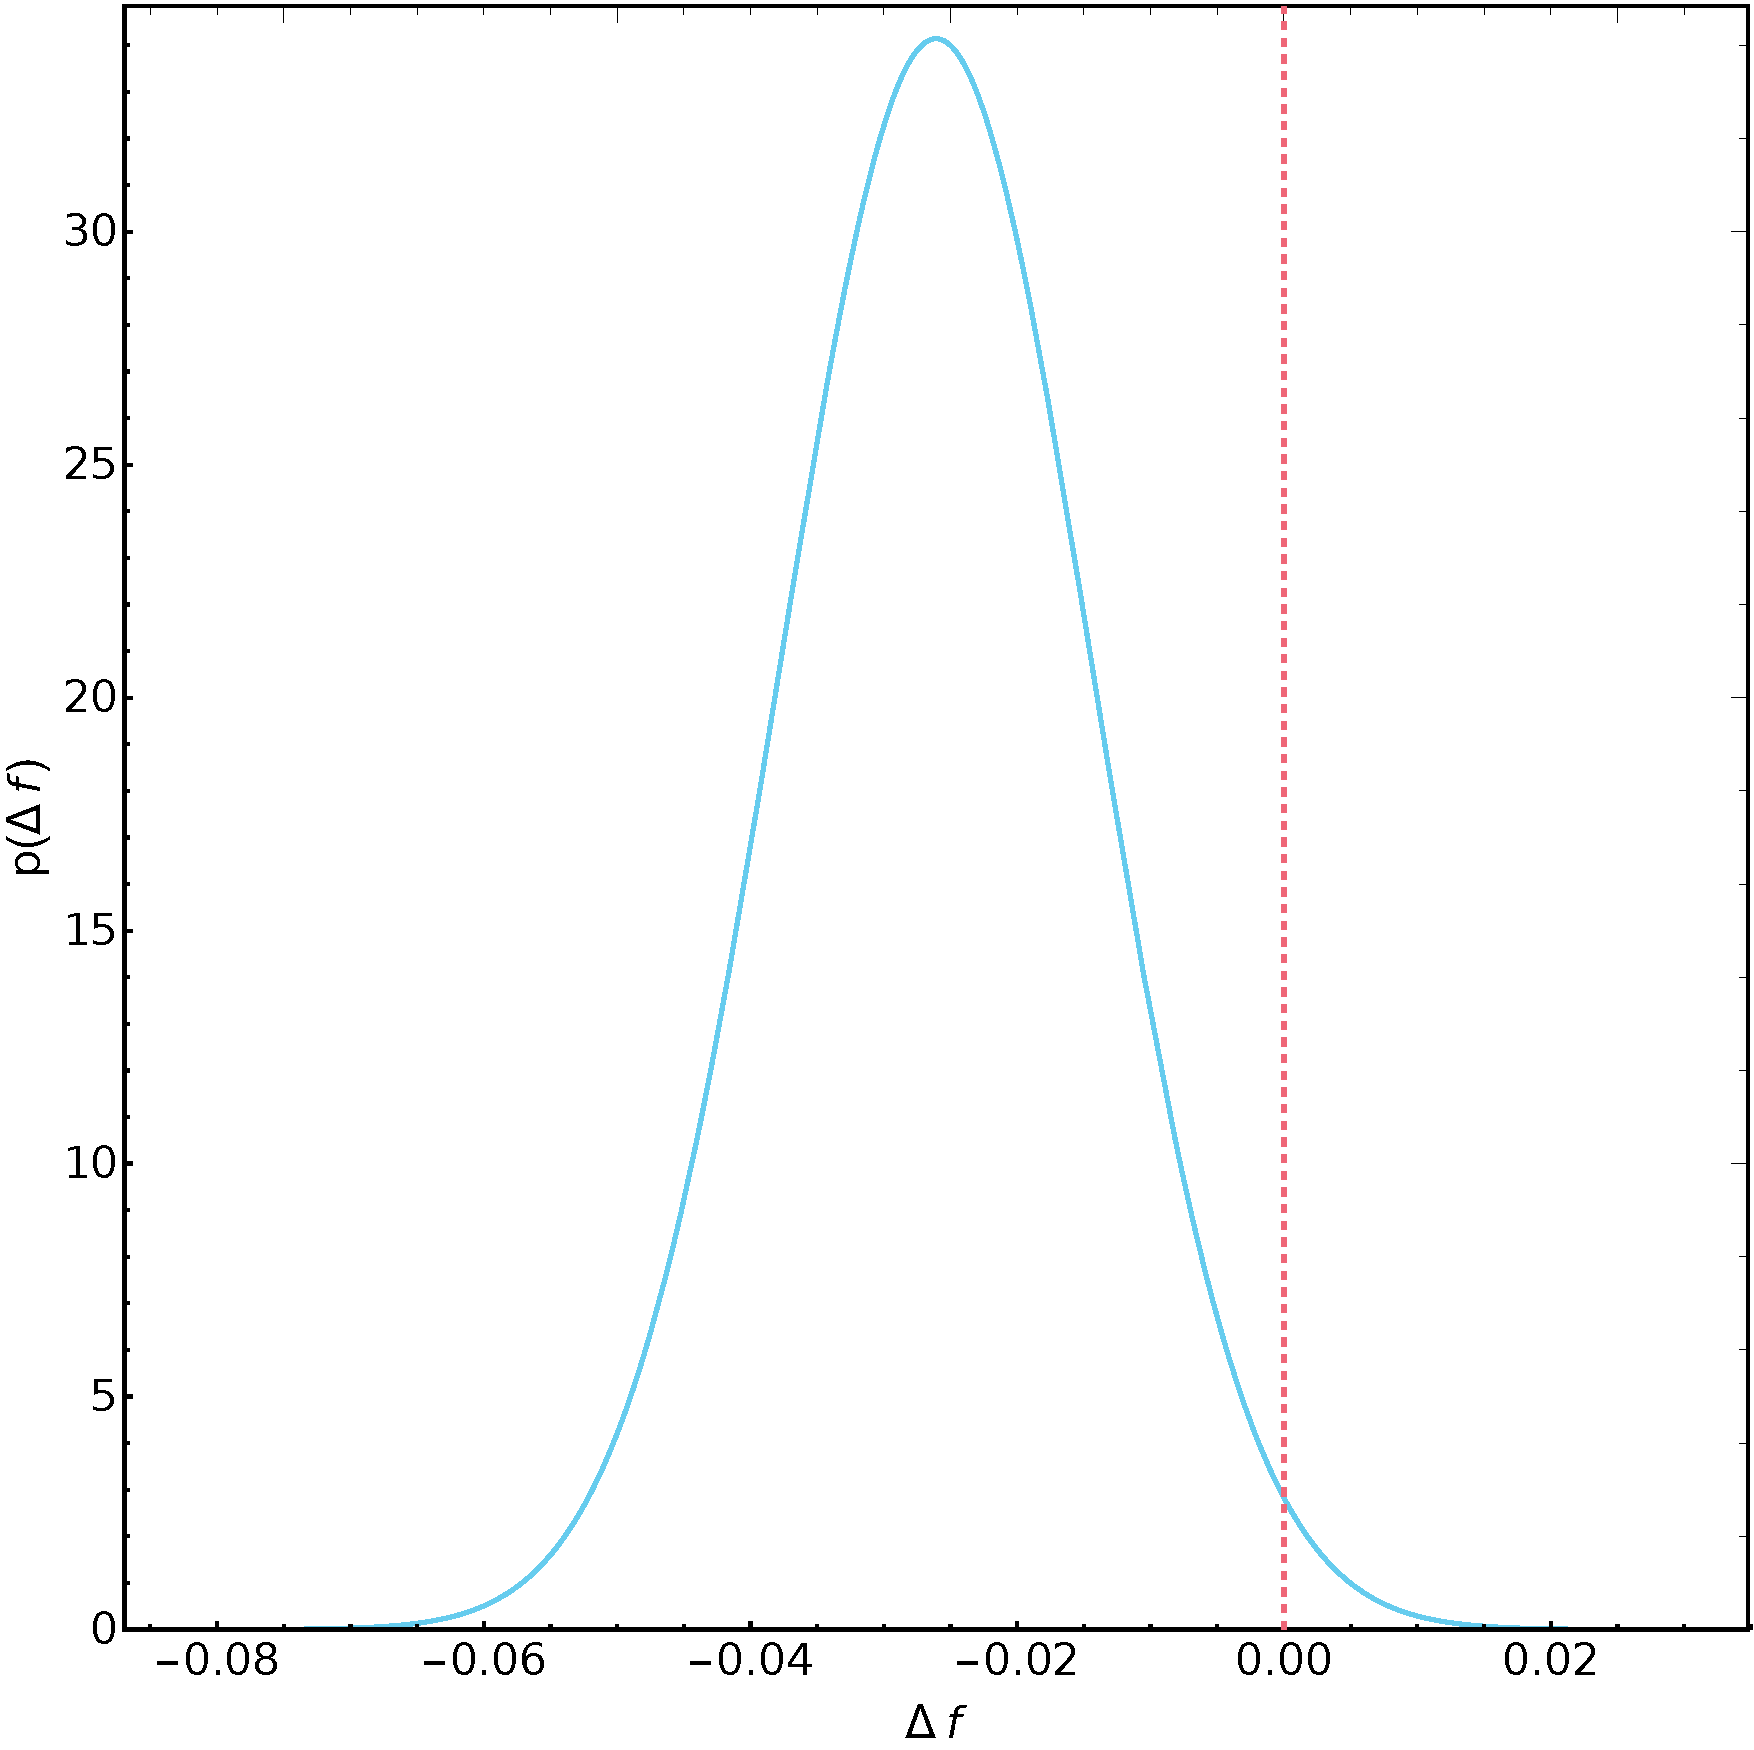
\includegraphics[width=0.49\linewidth]{example_diff.pdf}\hspace*{\stretch{1}}
 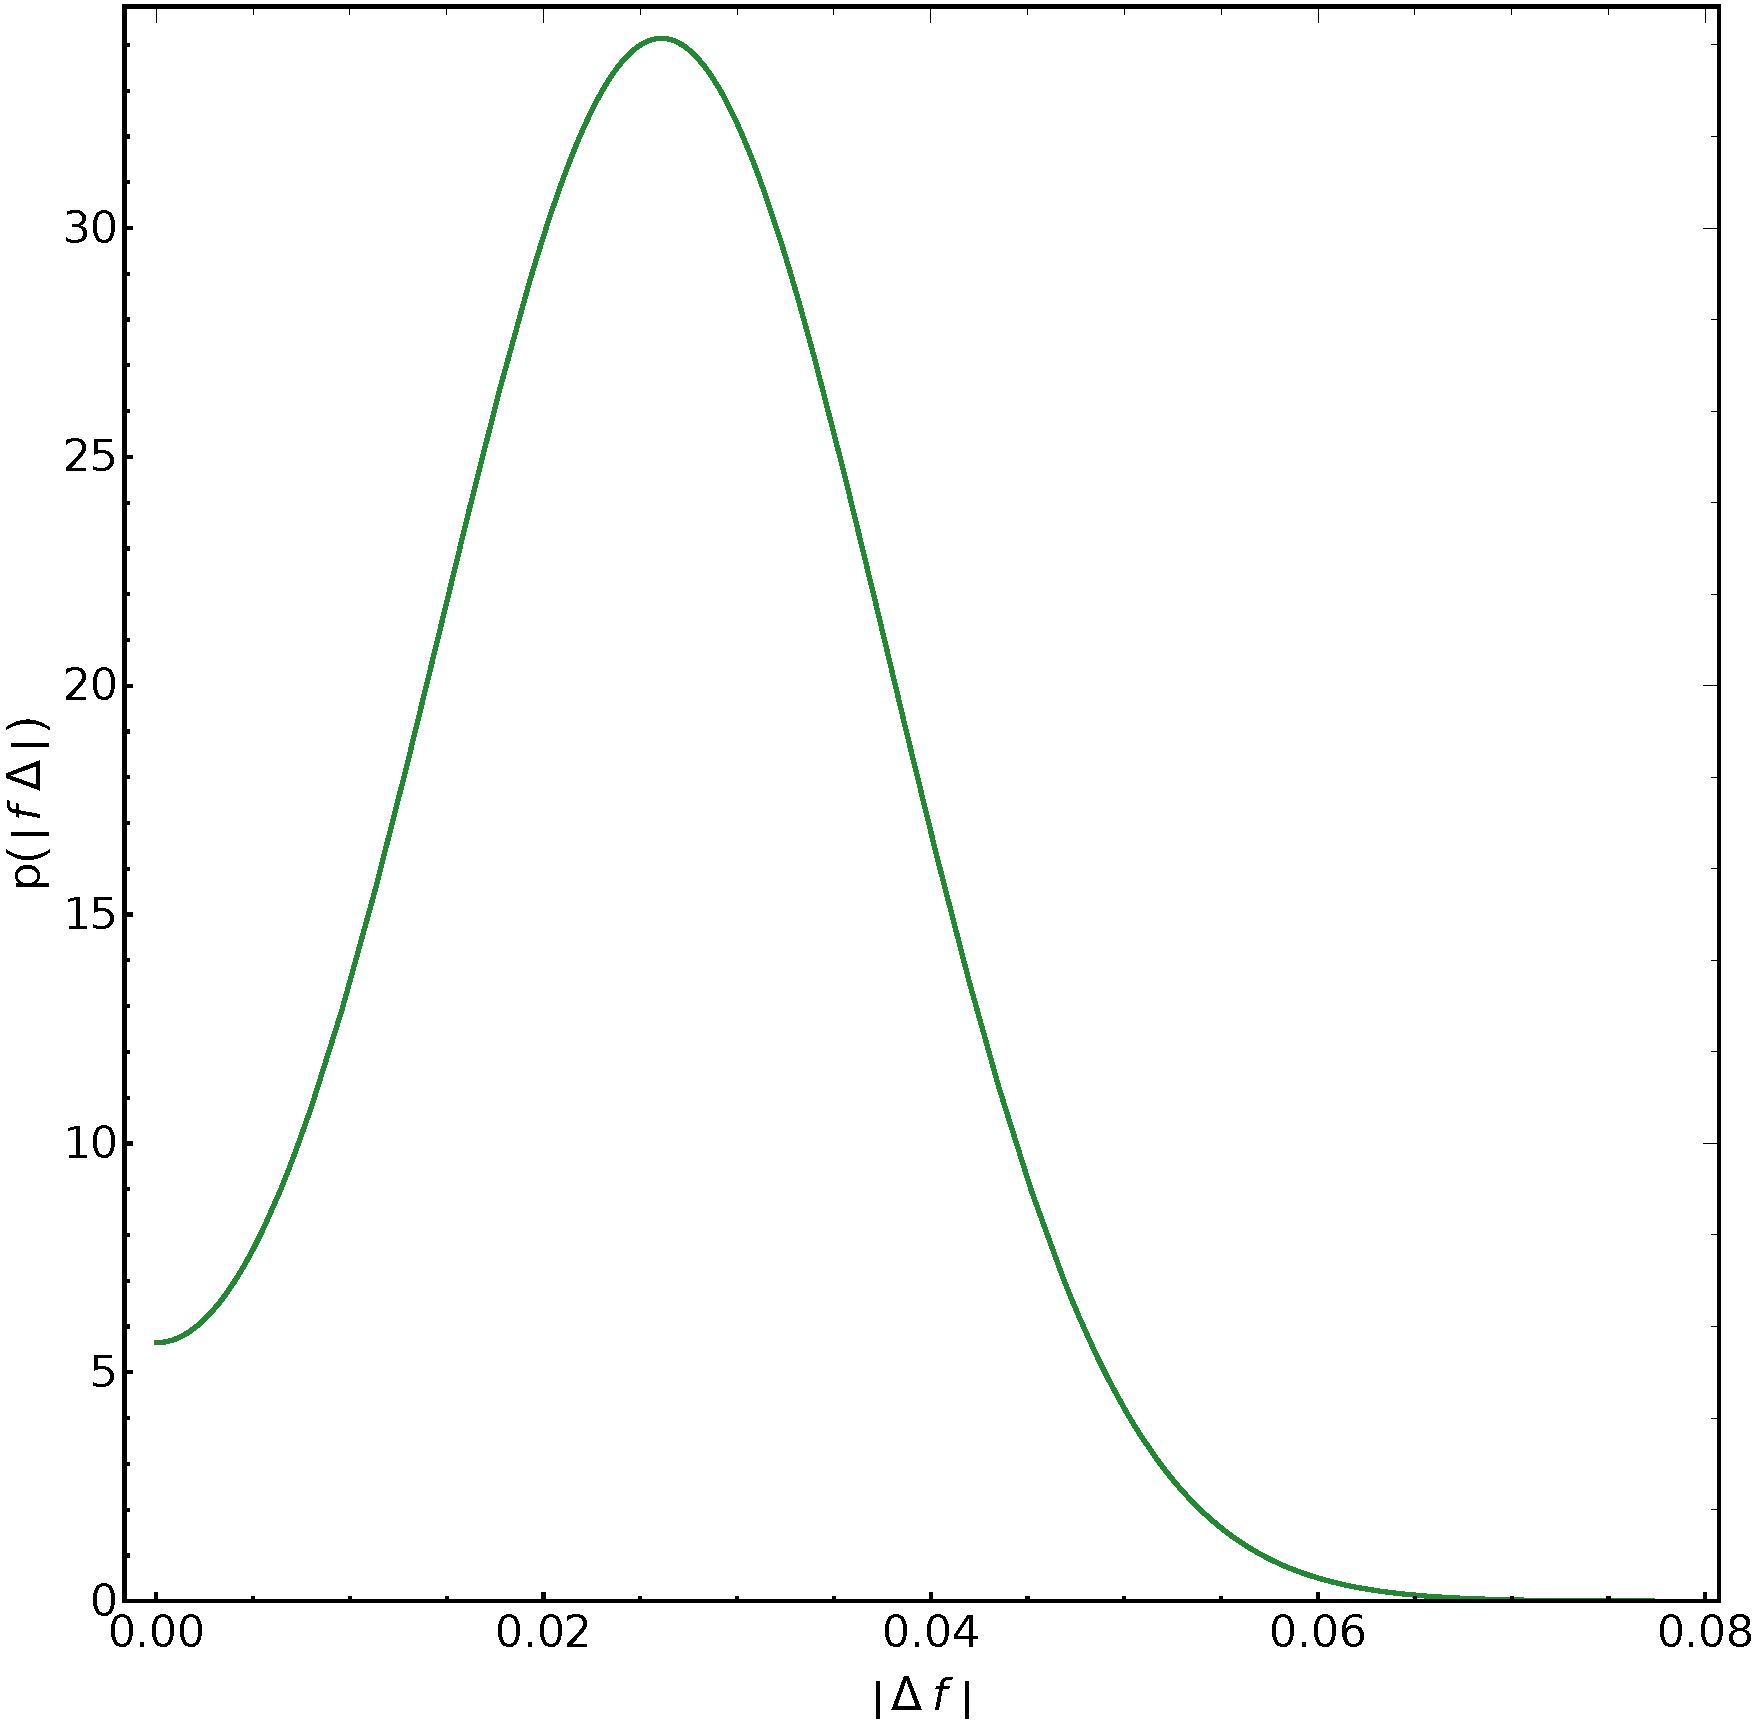
\includegraphics[width=0.75\linewidth]{example_absdiff.pdf}\\
 \caption{Example of probability distributions for $\abs{\df}$, the
   absolute difference between conditional frequencies.\mynote{add lines
     indicating the 10-quantile and
     expectation}}\label{fig:example_difference_distributions}
\end{figure}% scripts2/plot_curves.nb
% freq-1_1_conserv-spreads-sym_O-snp_6-spr_2.233.csv
% "spread_y",-2.23267970003192
% "EV_y",-0.0260880661493155
% "SD_y",0.0116846434125515

This distribution contains all probabilistic information we need, but we
can also try to summarize it with a single number. We can  for example
check what is the  minimal frequency difference we are
90\% sure about, that is, the lowest 10-quantile:
\begin{equation}\label{eq:significance_measure}
x\;\text{ such that }\; \pf(\abs{\df} > x)=0.9,
\end{equation}
or simply the expectation
\begin{equation}\label{eq:significance_measure_expabs}
  \E\bigl(\abs{\df}\bigr).
  % \equiv \sqrt{\frac{2}{\pu}}\sigma\exp\Biggl(-\frac{\mu^2}{2\sigma^2} \Biggr) + \mu \erf\Biggl( \frac{\mu}{\sqrt{2}\sigma} \Biggr),
\end{equation}
For the plot of \fig~\ref{fig:example_difference_distributions} such
measures are $0.0112$ and $0.0262$.
% values obtained in scripts2/plot_curves.nb
In this work we use the quantile measure~\eqref{eq:significance_measure},
but the results are the same if we use the expectation. \mynote{add maybe
  something about dependence of broadness on sample size, and
  \enquote{smoothing} as discussed by MacKay \amp\ Bauman Peto
  \citey[\sect~2.6]{mackayetal1995}.}

A more complete quantification of our plausible guesses is the joint
probability distribution $\pf(f_{|\ya}, f_{|\yb})$ for the two conditional
frequencies given the data and our pre-data assumptions, from which
$\pf(\df)$ can be calculated. This joint distribution is therefore the
pivot of our method in the next section.


\section{Method}
\label{sec:method}

\subsection{General plan}
\label{sec:inference}

To explain our method, consider a specific \snp\ with alleles $\ya$ and
$\yb$, and a specific insomnia symptom, for example $\ysO$. As announced in
the previous section, our calculations hinge on the joint probability for
the conditional frequencies of the symptom given the two alleles in a
hypothetical infinite population,
\begin{equation}
  \label{eq:goal_joint_prob}
  \pf(f_{|\ya}, f_{|\yb} \| \ptext{data}, \ptext{initial info}),
\end{equation}
conditional on the collected data an on our pre-data information or
assumptions.

The first step is to use Bayes's theorem:
\begin{multline}
  \label{eq:intuitive_Bayes}
  \pf(f_{|\ya}, f_{|\yb} \| \ptext{data}, \ptext{pre-data info})
  \propto{}\\
  \pf(\ptext{data} \| f_{|\ya}, f_{|\yb}, \ptext{pre-data info})
  \times
  \pf(f_{|\ya}, f_{|\yb} \| \ptext{pre-data info}),
\end{multline}
which says that we need to provide a probability and a probability
distribution:
\begin{enumerate*}[label=(\roman*)]
\item the probability of observing our data if we had known the
  conditional frequencies in the larger population; \item our pre-data
  probability distribution for the conditional frequencies.
\end{enumerate*}
The first is given by a sampling formula, calculated by counting. The
second can be modelled in several reasonable ways, but our data size is
large enough to make them all lead to very similar conclusions.

Once we have obtained the joint distribution~\eqref{eq:goal_joint_prob}, we
can calculate the probability distribution for the absolute frequency
difference, $\pf(\abs{\df} \| \ptext{data}, \ptext{pre-data info})$, by
standard methods, and from the latter we can compute our measure of link
strength~\eqref{eq:significance_measure}.


\subsection{Probability for the data given the frequencies}
\label{sec:p_data_from_freqs}

In our data we have $N_{\ya}$ individuals with allele $\ya$; of these, a
fraction $F_{|\ya}$ show the insomnia symptom of interest. For allele $\yb$
the number is $N_{\yb}$ and the fraction $F_{|\yb}$. The two fractions constitute
our data, while the total numbers are part of our pre-data information.

The probability of obtaining the data if we had known the frequencies in
the hypothetical infinite population can be calculated with a simple
\enquote{drawing with replacement} argument, which can be carried out for
each allele separately. It leads to a binomial distribution
\cites[\chap~3]{jaynes1994_r2003}[\sect~4.6]{ross1976_r2010}[\sect~VI.2]{feller1950_r1968}.
For allele $\ya$ we have
\begin{equation}
  \label{eq:sampling_belief}
  \pf( F_{|\ya} \| f_{|\ya}, \ptext{pre-data info})
  =
\binom{N_{\ya}}{N_{\ya}\,F_{|\ya}}\;  {f_{|\ya}}^{N_{\ya}\,F_{|\ya}} \;
  {(1-f_{|\ya})}^{N_{\ya}\,(1-F_{|\ya})},
\end{equation}
and analogously for allele $\yb$.

The probability for our full data set $(F_{|\ya},F_{|\yb})$ is therefore
the product of the binomials for the two alleles:
\begin{equation}
  \label{eq:sampling_belief_combined}
%  \pf(F_{|\ya},F_{|\yb} \|  f_{|\ya},f_{|\yb}, N_{\ya}, N_{\yb}, \yI)
  \pf(\ptext{data} \|  f_{|\ya},f_{|\yb}, \ptext{pre-data info})
  =
 \prod_{x=\ya,\yb} \binom{N_{x}}{N_{x}\,F_{|x}}\;{f_{|x}}^{N_{x}\,F_{|x}} \;
  {(1-f_{|x})}^{N_{x}\,(1-F_{|x})}.
\end{equation}

\subsection{Pre-data probability distribution for the frequencies}
\label{sec:p_initial}

Our pre-data belief distribution in the conditional relative frequencies
$f_{|\ya}$, $f_{|\yb}$ must be quantified with care, because it may play an
important part in our final probabilities if the effective size of the data
is small. We can assess the importance of our pre-data probability
distribution by considering several sensible alternative states of
knowledge and checking the difference of the results they lead to. In our
case we consider two alternatives.

\begin{figure}[t!]%{r}{0.4\linewidth} % with wrapfigure
 \centering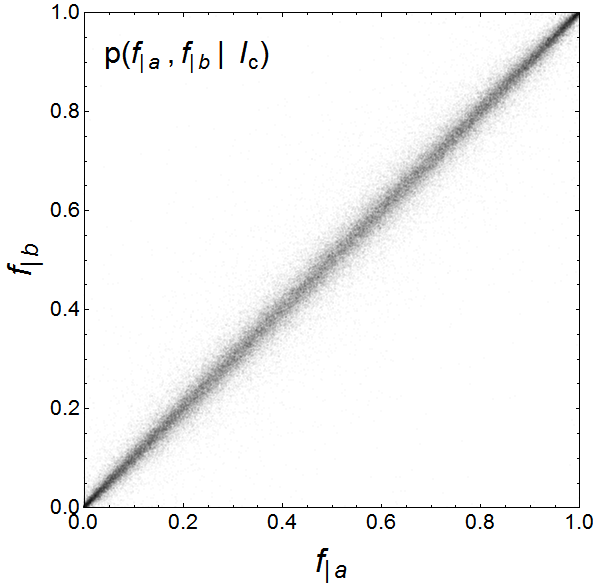
\includegraphics[width=0.49\linewidth]{conserv_prior_list.png}%
 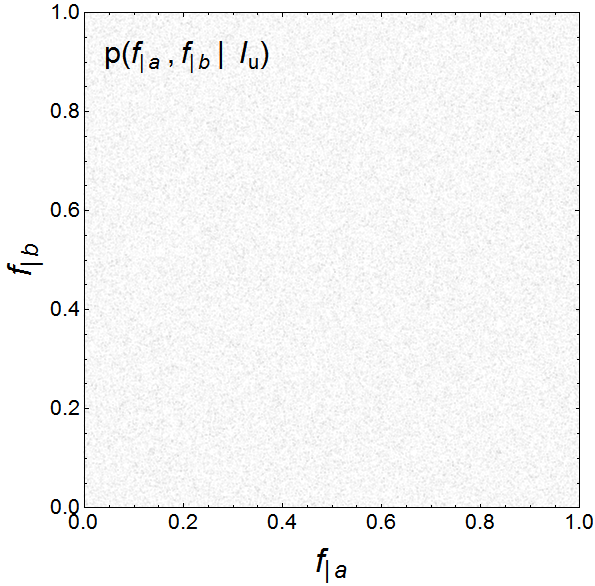
\includegraphics[width=0.49\linewidth]{unif_prior_list.png}
 \caption{Scatter plots of 100\,000 samples from two alternative states of
   knowledge. Left: more conservative state of knowledge $\yIc$
   (\eqn~\ref{eq:conservative_prior} in the Appendix); right: less
   conservative state of knowledge $\yIu$ (\eqn~\ref{eq:uniform_prior} in
   the Appendix).}\label{fig:initial_beliefs}
\end{figure}% scripts2/plot_priors.nb
The first, more conservative, is that we expect the two conditional
frequencies $f_{|\ya}$, $f_{|\yb}$ to be very similar. This implies some
degree of correlation between them. It also means that we don't expect, a
priori, any strong link between the \snp\ and the insomnia symptom under
analysis. This conservative state of knowledge, which we denote $\yIc$, is
represented as a scatter plot of sampled frequency pairs in the left panel
of \fig~\ref{fig:initial_beliefs}: we see that it's highly probable that
$f_{|\ya}$ and $f_{|\yb}$ have a similar value (high probability on the
diagonal), although we are completely uncertain about what the value should
be (almost uniform probability within the diagonal). Note that this state
of knowledge is quite conservative; if our post-data joint distribution
nevertheless shows very distinct conditional frequencies, it means that the
data have such strong evidence for this difference as to overwhelm this
conservative state of knowledge.

The second, less conservative, is that we do not expect any correlation
between the two conditional frequencies. This means that we don't exclude
the possibility of a strong link between the \snp\ and the insomnia
symptom. This state of knowledge, which we call \enquote{uniform} (as its
distribution) and denote by $\yIu$ , is represented in the right panel of
\fig~\ref{fig:initial_beliefs}: we see that all possible pairs of values
are equally probable.

The mathematical expression of these two states of knowledge is discussed in
the Appendix. Here we mention that the more conservative state of knowledge
$\yIc$ can also be interpreted as so-called \emph{hierarchic}
model\citep[for example][]{good1980}, and that it corresponds to the
technique of \emph{shrinkage} in the probability literature, used in a
variety of association studies, from
genetics\citep{lange1995,lockwoodetal2001} to contextual text
prediction\citep{mackayetal1995} and even baseball\citep{jiangetal2010}.

\subsection{Post-data probability distribution for the frequencies}
\label{sec:p_final}

We now have the probability~\eqref{eq:sampling_belief} for the data, and
two pre-data probability distributions, \fig~\ref{fig:initial_beliefs}, for
the frequencies. We can plug them in Bayes's
theorem~\eqref{eq:intuitive_Bayes} to obtain our post-data probability
distribution for the pairs of conditional frequencies. As an example, the
results for onset insomnia $\ysO$ and the \snp\ \texttt{rs875994} are shown
in \fig~\ref{fig:final_beliefs}. The left panel shows our inference for the
more conservative pre-data state of knowledge $\yIc$, and the right panel
for the less conservative one $\yIu$.
\begin{figure}[t!]%{r}{0.4\linewidth} % with wrapfigure
 \centering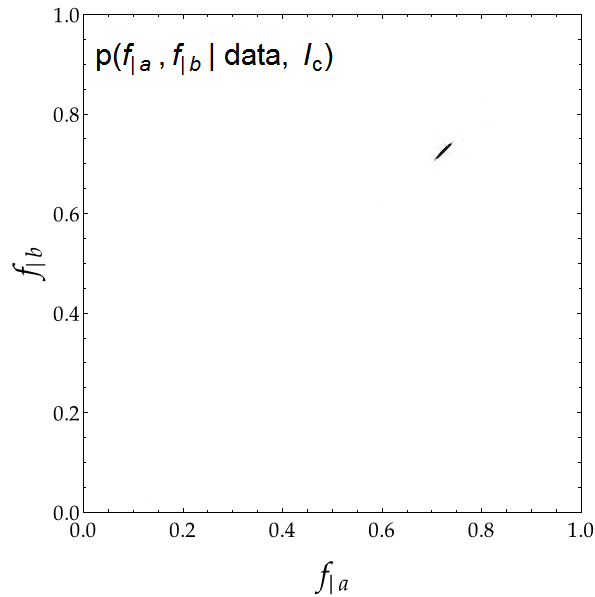
\includegraphics[width=0.49\linewidth]{cons_post_list.png}%
 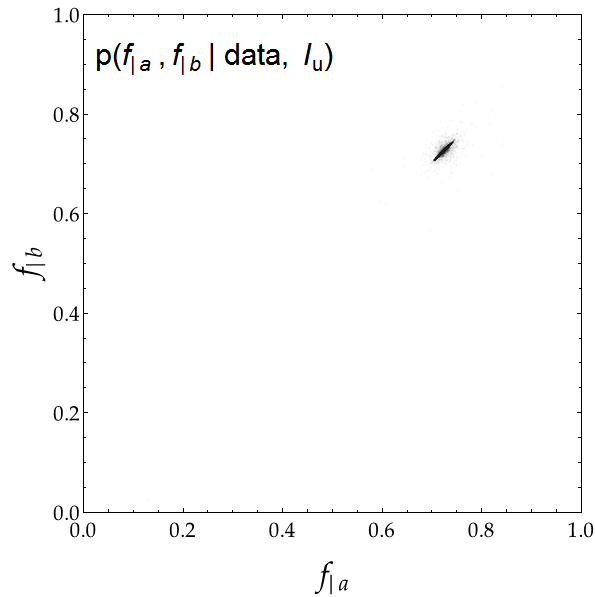
\includegraphics[width=0.49\linewidth]{unif_post_list.png}
 \caption{Scatter plots of 10\,000 samples from the post-data probability
   distribution for the frequencies of onset insomnia $\ysO$ conditional on
   the alleles of \snp\ \texttt{rs875994}%_C
   (first \snp\ in \fig~\ref{fig:relevance_sorted}), relative to the two
   alternative states of knowledge. Left: more conservative state of
   knowledge $\yIc$; right: less conservative state of knowledge
   $\yIu$.}\label{fig:final_beliefs}
\end{figure}
% scripts2/plot_posteriors.nb
% scripts2/example_joint_posterior.R
% scripts2/conditional_freqs_2.R
In both cases the probability mass appears to be very close to the
diagonal, but a more precise calculation reveals that it's more than 90\%
probable that the absolute difference of the conditional frequencies
$\abs{\df}$ is larger than $0.01$.

From the joint distribution above we can find, with a routine calculation,
the distribution for the absolute value of the difference of the two
frequencies $\pf(\abs{\df} \| \ptext{data}, \ptext{pre-data info})$ and its
10-quantile, our measure~\eqref{eq:significance_measure}. Such quantiles
are shown, sorted, in \fig~\ref{fig:relevance_sorted} for all \snp-symptom
pairs. For each pair we show the result for the two pre-data states of
knowledge, joined by a line.

\section{Results}
\label{sec:results}

\mynote{discussion of the possible biological connection between the topmost 5--6
  \snp s of \fig~\ref{fig:relevance_sorted} and insomnia}

% \begin{figure}[p!]%{r}{0.4\linewidth} % with wrapfigure
%  \centering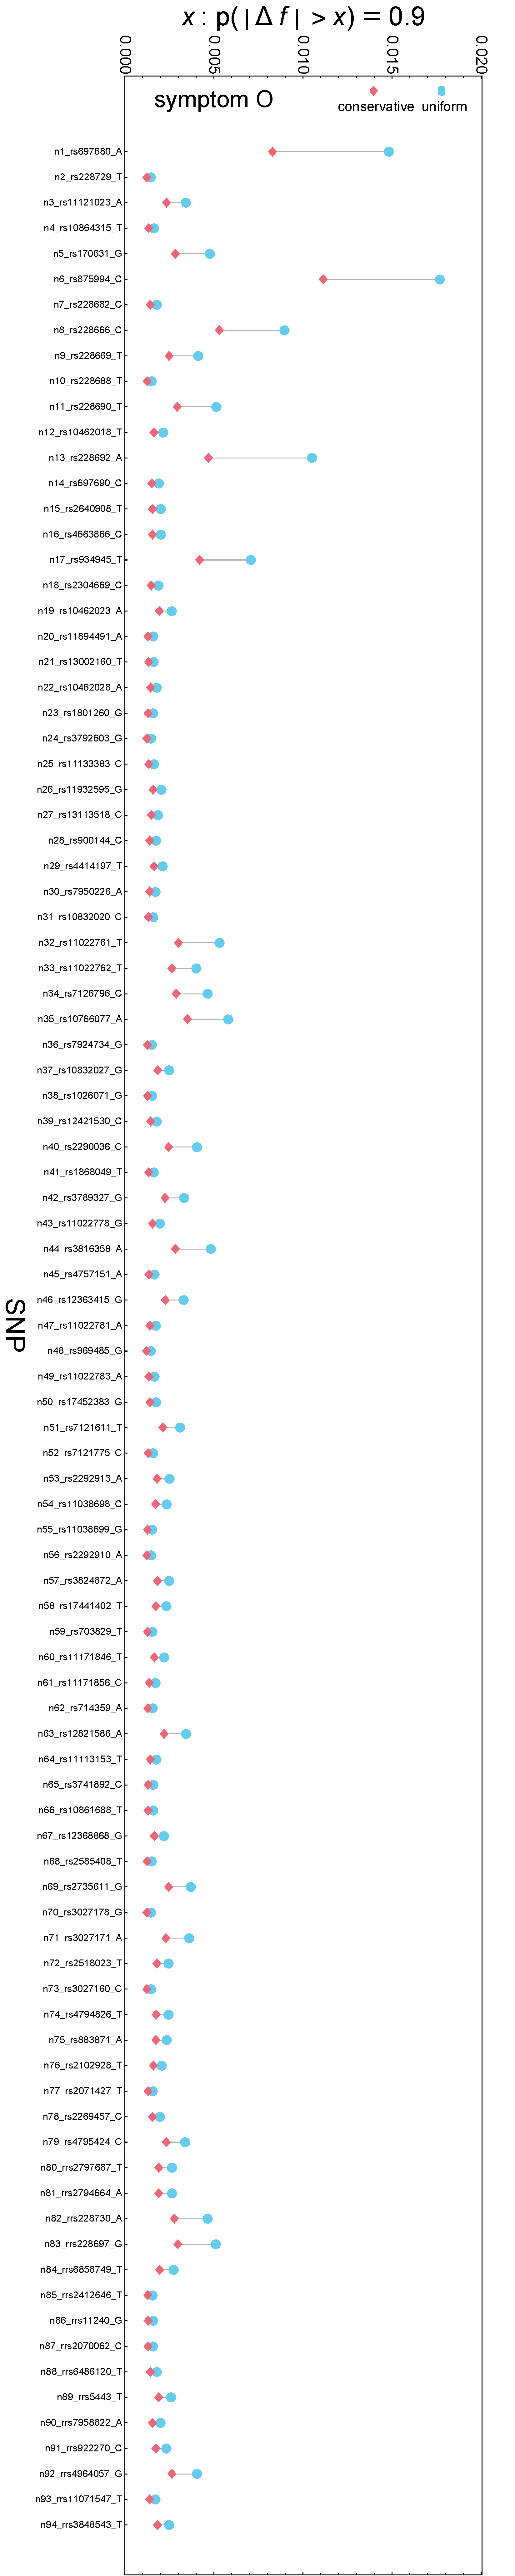
\includegraphics[height=\textheight]{x90-sym_O.pdf}\hspace*{\stretch{1}}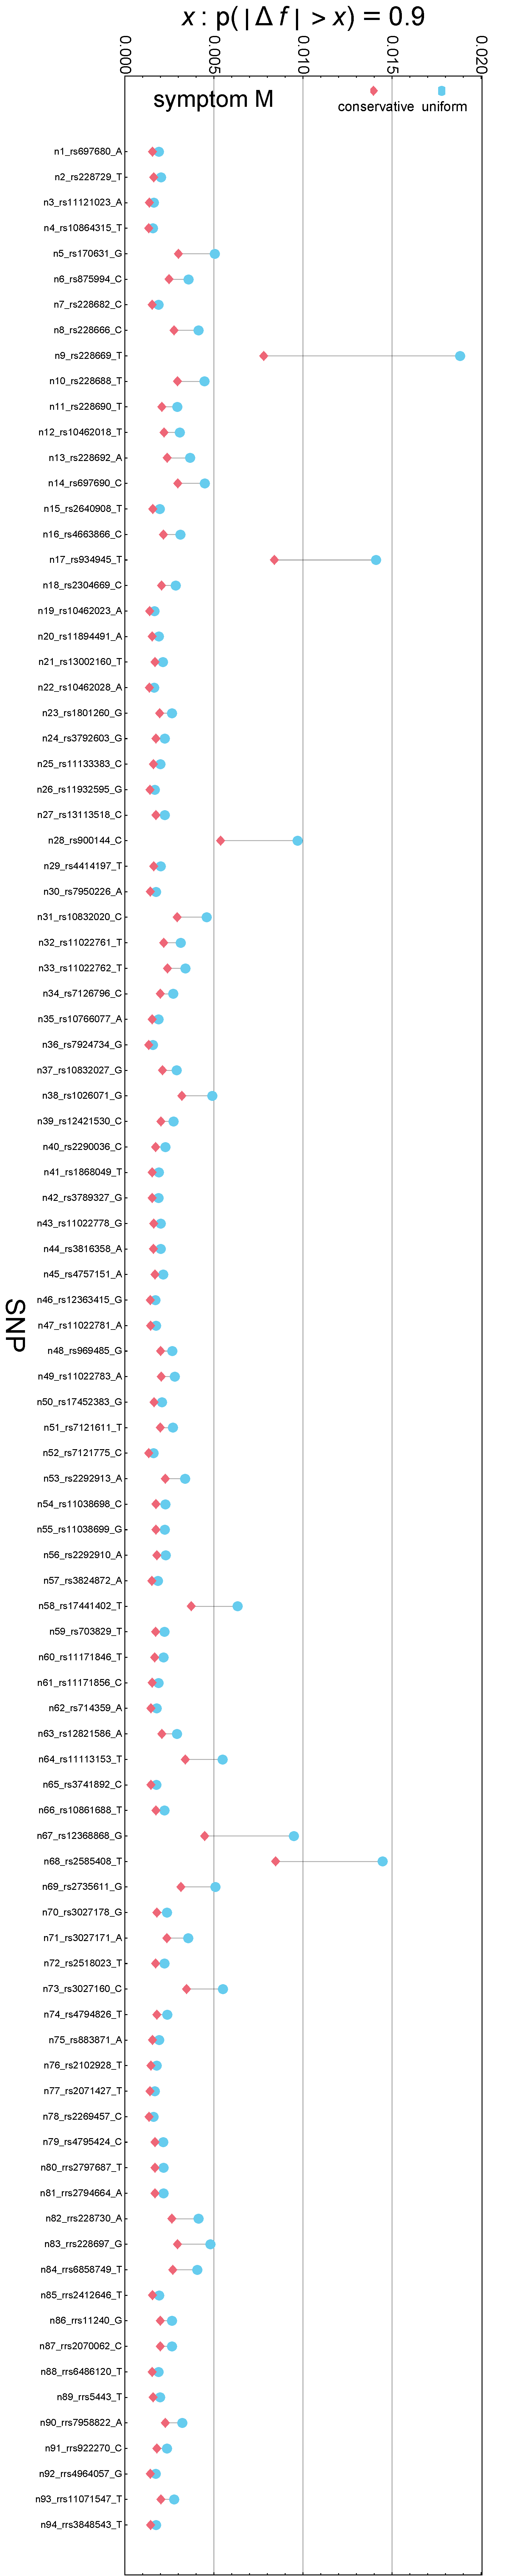
\includegraphics[height=\textheight]{x90-sym_M.pdf}\hspace*{\stretch{1}}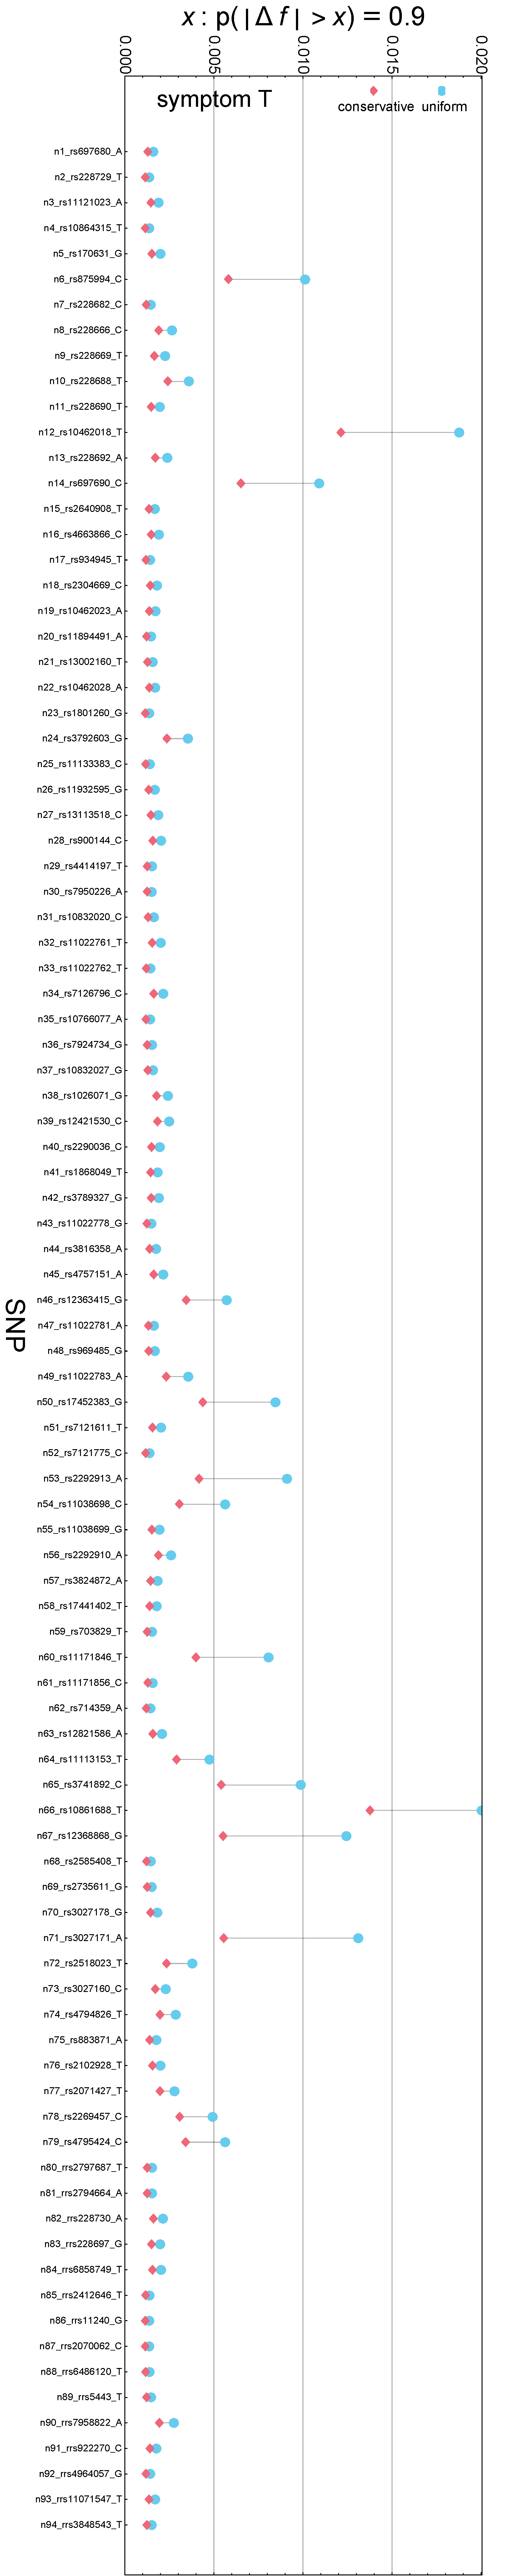
\includegraphics[height=\textheight]{x90-sym_T.pdf}\\
% \caption{\enquote{Relevance} of the 94 \snp s for the three symptoms.}\label{fig:not-relevance}
% \end{figure}% scripts2/plot_results.nb

\begin{figure}[p!]%{r}{0.4\linewidth} % with wrapfigure
 \centering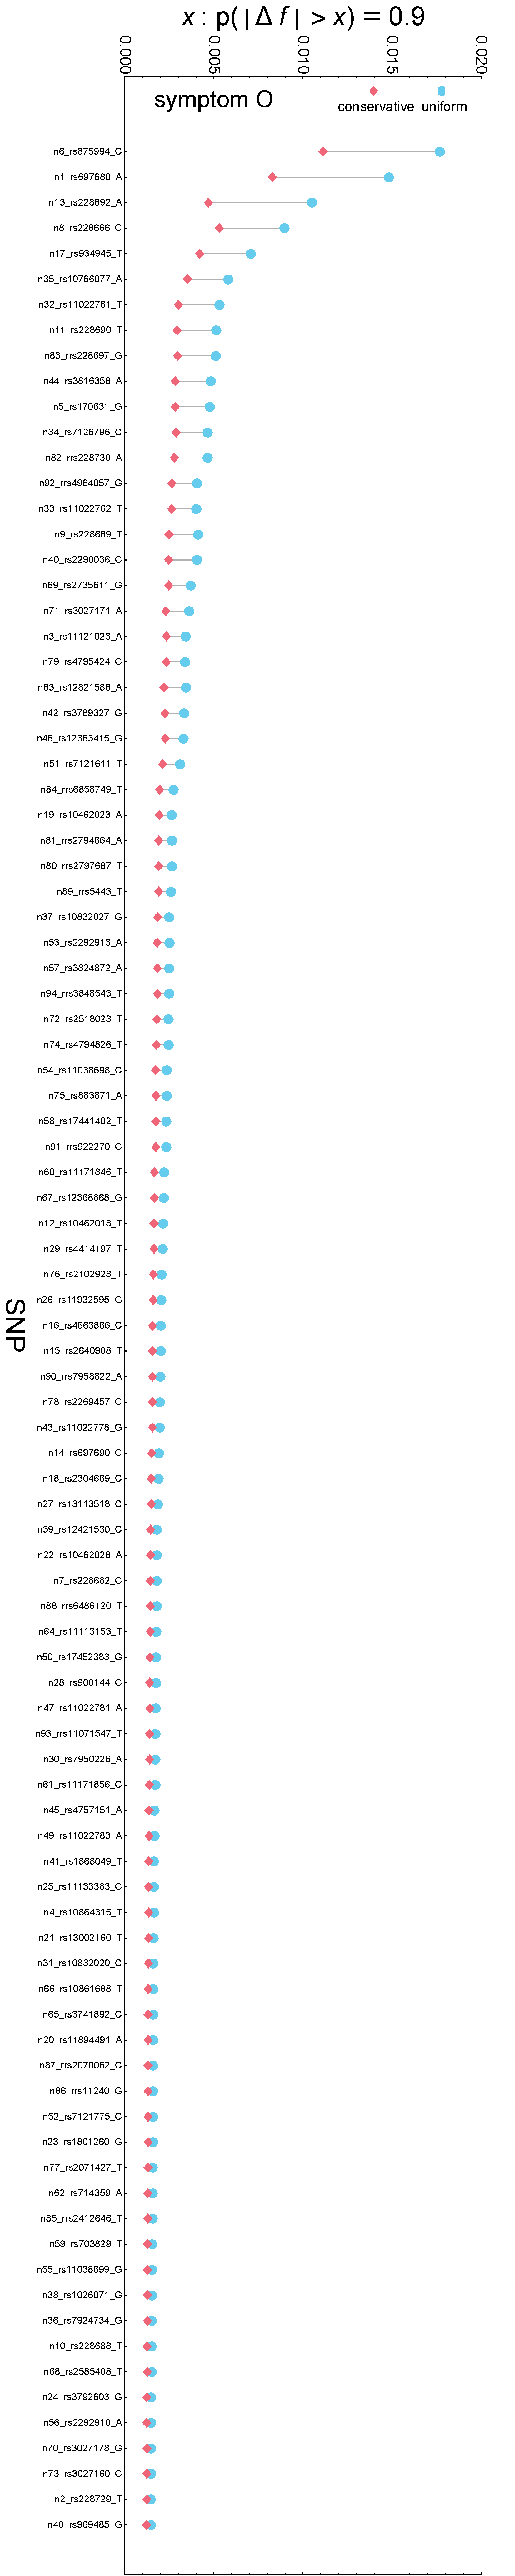
\includegraphics[height=\textheight]{x90sort-sym_O.pdf}\hspace*{\stretch{1}}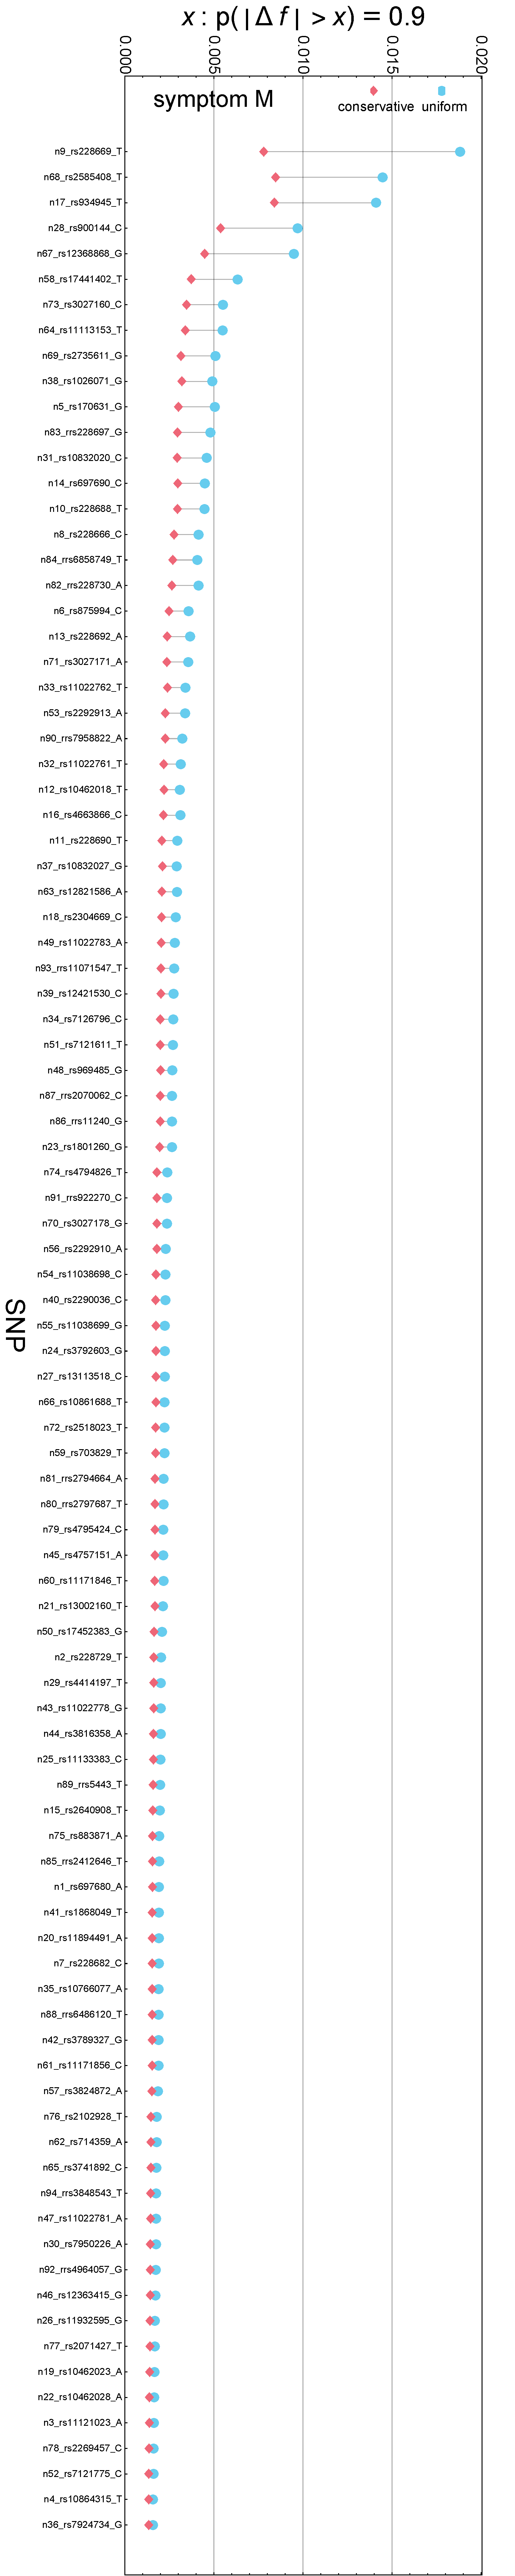
\includegraphics[height=\textheight]{x90sort-sym_M.pdf}\hspace*{\stretch{1}}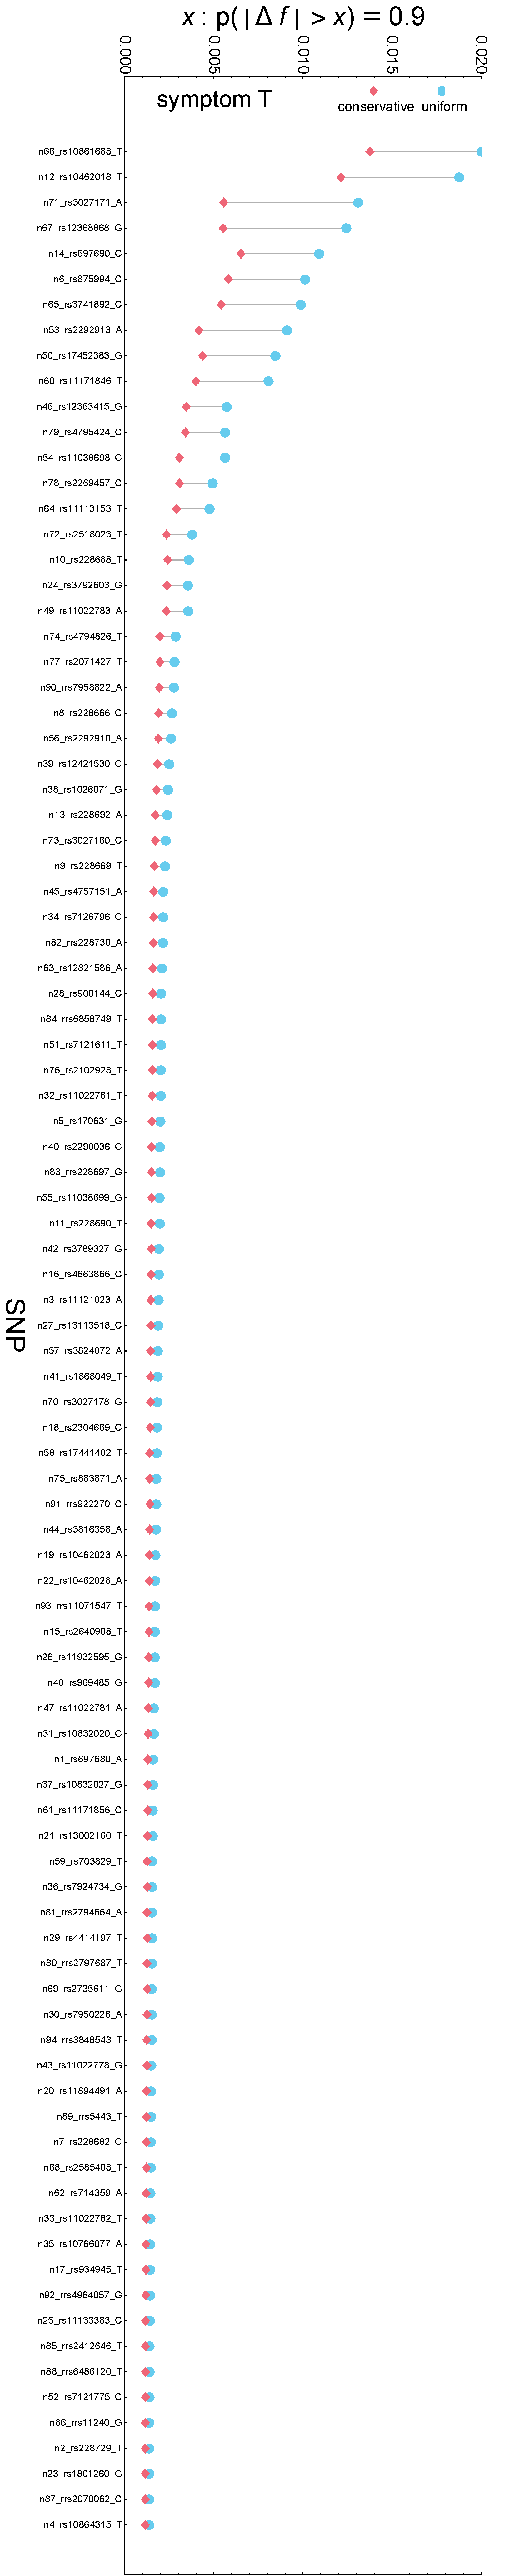
\includegraphics[height=\textheight]{x90sort-sym_T.pdf}\\
 \caption{Link strength, measured with
   formula~\eqref{eq:significance_measure}, of the 94 \snp s for the three
   symptoms.}\label{fig:relevance_sorted}
\end{figure}% scripts2/plot_results.nb

\newpage
\renewcommand*{\appendixpagename}{Appendix}
\renewcommand*{\appendixname}{Appendix}
%\appendixpage
\appendix
\setcounter{section}{1}%\renewcommand*{\thesection}{\Alph{section}}

\subsection{Pre-data plausibility distributions for the frequencies}
\label{sec:p_initial}

The pre-data probability density shown in the right panel of
\fig~\ref{fig:initial_beliefs} is uniform in the two conditional
frequencies (that is, with respect to the base density
$\di f_{|\ya}\,\di f_{|\yb}$):
\begin{equation}
  \label{eq:uniform_prior}
  \pf(f_{|\ya}, f_{|\yb} \| \yIu)%\;\di f_{|\ya}\,\di f_{|\yb}
  =1.%\di f_{|\ya}\,\di f_{|\yb}.
\end{equation}

The more conservative density in the left panel of the same figure has this
mathematical expression:
\begin{subequations}
  \label{eq:conservative_prior}
  \begin{gather}
    \pf(f_{|\ya}, f_{|\yb} \| \yIc)%\;\di f_{|\ya}\,\di f_{|\yb}
    =
    \int_{\mathrlap{0}}^{\mathrlap{\infty}}\di\yua
    \int_{\mathrlap{0}}^{\mathrlap{\infty}}\di\yub\;
    \pf(f_{|\ya}, f_{|\yb} \| \yua,\yub,\yIc)\;
    \pf(\yua,\yub \| \yIc)%\;\di f_{|\ya}\,\di f_{|\yb}
    \\
    \shortintertext{with}
    \label{eq:beta_product}
    \pf(f_{|\ya}, f_{|\yb} \| \yua,\yub,\yIc)\defd
    \dbeta(f_{|\ya} \| \yua,\yub)\;
    \dbeta(f_{|\yb} \| \yua,\yub),
    \\
    \label{eq:p_initial_parameters}
    \pf(\yua,\yub \| \yIc)\defd \frac{1}{u+v}\,\dgamma(u+v \| 1, 1000)
  \end{gather}
  where $\dbeta$ and $\dgamma$ are beta and gamma densities:
  \begin{gather}
    \label{eq:def_beta}
    \dbeta(f \| \yua,\yub) \defd
    \frac{\Gamma(\yua+\yub)}{\Gamma(\yua)\,\Gamma(\yub)}\;
    f^{\yua-1}\;(1-f)^{\yub-1},
    \qquad  \yua,\yub>0,
    \\
    \label{eq:def_gamma}
    \dgamma(\yA \| 1, 1000) \defd
    \frac{1}{1000}\,\exp(-\yA/1000).
  \end{gather}
\end{subequations}
The integral expression above can be interpreted as follows: we consider
several joint probability distributions for the two frequencies; each
distribution being the product of two beta densities with identical shape
parameters. All these distributions are weighted and mixed together; their
mixture expresses a belief that is \emph{not} independent in the two
frequencies. This is a simple example of a hierarchic model\citep[for
example][]{good1980}.

The weights of the mixture are given by a gamma density. The use of beta
densities in this problem seems to have been first endorsed by G. F.
Hardy\citep{hardy1889}; Good\citep[\sect~4.1]{good1965}[\sect~4]{good1980}
motivates the use of their mixtures. The specific shape and scale values of
the gamma density are so chosen as to concentrate our initial belief along
the $(f_{|\ya}, f_{|\yb})$ diagonal. 

\subsection{Final plausibilities}
\label{sec:p_final}

In the case of the uniform pre-data state of knowledge $\yIu$,
multiplication of the probability for the
data~\eqref{eq:sampling_belief_combined} and the pre-data
density~\eqref{eq:uniform_prior} leads to a density for the frequencies
proportional to the product of two beta densities. Our final density in
this case is
\begin{equation}
  \label{eq:final_from_uniform}
  \pf(f_{|\ya}, f_{|\yb} \| \yD, \yIu)
  =
\prod_{x=\ya,\yb}
\dbeta[f_{|x} \| N_{x}\,F_{|x}+1, N_{x}\,(1-F_{|x})+1]
% \frac{\Gamma(N_{x}\,F_{|x}+1)\,\Gamma[N_{x}\,(1-F_{|x})+1]}{
%   \Gamma(N_{x}+2)}\;
% {f_{|x}}^{N_{x}\,F_{|x}} \;  {(1-f_{|x})}^{N_{x}\,(1-F_{|x})}.
\end{equation}
This is the product of two independent densities for the frequencies.

In the case of the conservative pre-data state of knowledge $\yIc$,
multiplication of~\eqref{eq:sampling_belief_combined} and the beta
densities within the integral of \eqn~\eqref{eq:conservative_prior} leads
to two new unnormalized beta densities. Grouping the normalization constant
with the density for the parameters~\eqref{eq:p_initial_parameters} yields
a final density in integral form:
\begin{subequations}
  \label{eq:final_from_conservative}
  \begin{gather}
  \begin{multlined}[t][\linewidth]
    \pf(f_{|\ya}, f_{|\yb} \| \yD, \yIc)
    ={}\\[\jot]
    \int_{\mathrlap{0}}^{\mathrlap{\infty}}\di\yua
    \int_{\mathrlap{0}}^{\mathrlap{\infty}}\di\yub\,
    \prod_{x=\ya,\yb}\Bigl\{ 
    \dbeta\bigl[f_{|x} \| N_{x}\,F_{|x} +\yua, N_{x}\,(1-F_{|x})+\yub\bigr]
    \Bigr\}\; \pf(\yua,\yub \| \yD,\yIc)
  \end{multlined}\\
  \shortintertext{with}
      \label{eq:posterior_parameters}
  \begin{multlined}[t][\linewidth]
    \pf(\yua,\yub \| \yD,\yIc) \propto{}\\[\jot]
    \prod_{x=\ya,\yb}\left\{
      \frac{\Gamma(N_{x}\,F_{|x}+\yua)\;\Gamma[N_{x}\,(1-F_{|x})+\yub]}
      {\Gamma(N_{x}+\yua+\yub)}\,
      \frac{\Gamma(\yua+\yub)}
      {\Gamma(\yua)\;\Gamma(\yub)} \right\}
    \,\frac{\dgamma(\yua+\yub \| 1, 1000)}{\yua+\yub}.
  \end{multlined}
\end{gather}
\end{subequations}
This density also has a hierarchic form. The integral doesn't have an
closed form, but the final density for the frequencies can be sampled by
generating samples of the shape parameters $\yua$, $\yub$
from~\eqref{eq:posterior_parameters} via Markov-Chain Monte Carlo methods,
and for each generating samples of the frequencies from the beta densities
with those shape parameters (alternatively we can write an averaged sum of
beta distributions having the sampled shape parameters). For this study we
used an automated-factor slice sampler\citep{hall2014}.

\subsection{Final calculation of the link strength}
\label{sec:calc_link}

The final densities~\eqref{eq:final_from_uniform}
and~\eqref{eq:final_from_conservative} above can be well approximated by
normal densities. We only need to determine their means and covariance
matrices. These can be easily calculated using the first and second raw
moments of a beta distribution:\mynote{refs for this}
\begin{equation}
  \label{eq:moments_beta}
  \E(f \| \yua,\yub) = \frac{\yua}{\yua+\yub},
  \qquad
  \E(f^2 \| \yua,\yub) = \frac{\yua\,(\yua+1)}{(\yua+\yub)\,(\yua+\yub+1)}.  
\end{equation}


For the uniform initial state of knowledge~\eqref{eq:final_from_uniform}
the means, variances, and covariance are readily calculated:
\begin{subequations}
  \label{eq:stats_final_unif}
  \begin{align}
    \label{eq:mean_final_unif}
    &\E(f_{|x}\| \yD, \yIu) =
    \frac{N_{x}\,F_{|x}+1}{N_{x}+2},
    \frac{N_{\yb}\,F_{|\yb}+1}{N_{\yb}+2}
    \qquad x=\ya,\yb,
    \\
    \label{eq:var_final_unif}
    &\var(f_{|x} \| \yD, \yIu) =
    \frac{(N_{x}F_{|x}+1)\,[N_{x}\,(1-F_{|x})+1)}{(N_{x}+2)^2\,(N_{x}+3)}
    \qquad x=\ya,\yb,
    \\
    \label{eq:cov_final_unif}
    &\cov(f_{|\ya}, f_{|\yb} \| \yD, \yIu) = 0.
    % \begin{pmatrix}
    %   \frac{(N_{\ya}F_{|\ya}+1)\,[N_{\ya}\,(1-F_{|\ya})+1)}{(N_{\ya}+2)^2\,(N_{\ya}+3)}
    %   &0\\0&
    %   \frac{(N_{\yb}F_{|\yb}+1)\,[N_{\yb}\,(1-F_{|\yb})+1)}{(N_{\yb}+2)^2\,(N_{\yb}+3)}
    % \end{pmatrix}.
  \end{align}
\end{subequations}
The covariance vanishes owing to the product form of the final density.

For the conservative initial state of
knowledge~\eqref{eq:final_from_conservative} let us first introduce the
notation
\begin{equation}
  \label{eq:notation_avg_parameters}
  \uav{X(\yua,\yub)} \defd
      \int_{\mathrlap{0}}^{\mathrlap{\infty}}\di\yua
    \int_{\mathrlap{0}}^{\mathrlap{\infty}}\di\yub\,
X(\yua,\yub) \, \pf(\yua,\yub \| \yD,\yIc);
\end{equation}
such an average can approximately be computed by averaging from a Monte
Carlo sample. The means, variances, and covariance of the final density are
\begin{subequations}
  \label{eq:stats_final_conserv}
  \begin{align}
    \label{eq:mean_final_conserv}
    &\E(f_{|x} \| \yD, \yIc) =
                                 \uav{\frac{N_{x}\,F_{|x}+\yua}{N_{x}+\yua+\yub}}
                                 \qquad x=\ya,\yb,
\\
  \label{eq:var_final_conserv}
    &\!\begin{multlined}[\linewidth]
\var(f_{|x} \| \yD, \yIc) =
  \uav{\frac{(N_{x}F_{|x}+\yua)\,(N_{x}F_{|x}+\yua+1)}{(N_{x}+\yua+\yub)\,(N_{x}+\yua+\yub+1)}}
  -
  \uav{\frac{N_{x}\,F_{|x}+\yua}{N_{x}+\yua+\yub}}^2
  \\ x=\ya,\yb  
\end{multlined}
    \\
    \label{eq:cov_final_conserv}
&    \cov(f_{|\ya}, f_{|\yb} \| \yD, \yIc) =
    \uav{\prod_{x=\ya,\yb}\frac{N_{x}\,F_{|x}+\yua}{N_{x}+\yua+\yub}}
    - \prod_{x=\ya,\yb}
    \uav{\frac{N_{x}\,F_{|x}+\yua}{N_{x}+\yua+\yub}}.
% &\!\begin{multlined}[\linewidth]
%     \cov(f_{|\ya}, f_{|\yb} \| \yD, \yIu) ={}\\[\jot]
%     \uav{\frac{N_{\ya}\,F_{|\ya}+\yua}{N_{\ya}+\yua+\yub}\,
%       \frac{N_{\yb}\,F_{|\yb}+\yua}{N_{\yb}+\yua+\yub}}
%     -
%     \uav{\frac{N_{\ya}\,F_{|\ya}+\yua}{N_{\ya}+\yua+\yub}}\,
%     \uav{\frac{N_{\yb}\,F_{|\yb}+\yua}{N_{\yb}+\yua+\yub}}.
%   \end{multlined}
  \end{align}
\end{subequations}
The covariance does not vanish owing to our initial correlated beliefs
about the two conditional frequencies.

It is worth remarking that for our data sample the typical average values
of the shape parameters $\uav{\yua}$, $\uav{\yub}$ are comparable to the
sample size $N_{\ya}+N_{\yb}$. Trying an expansion of
formulae~\eqref{eq:stats_final_conserv} around the uniform
formulae~\eqref{eq:stats_final_unif} in powers of $\uav{\yua}$,
$\uav{\yub}$ is therefore prone to produce bad approximations.




%%\setlength{\intextsep}{0.5ex}% with wrapfigure
%\begin{figure}[p!]%{r}{0.4\linewidth} % with wrapfigure
%  \centering\includegraphics[trim={12ex 0 18ex 0},clip,width=\linewidth]{maxent_saddle.png}\\
%\caption{caption}\label{fig:not-comparison_a5}
%\end{figure}% exp_family_maxent.nb


%%%%%%%%%%%%%%%%%%%%%%%%%%%%%%%%%%%%%%%%%%%%%%%%%%%%%%%%%%%%%%%%%%%%%%%%%%%%
%%% Acknowledgements
%%%%%%%%%%%%%%%%%%%%%%%%%%%%%%%%%%%%%%%%%%%%%%%%%%%%%%%%%%%%%%%%%%%%%%%%%%%% 
%\iffalse
\begin{acknowledgements}
  PGLPM thanks Mari \amp\ Miri for continuous encouragement and affection;
  Buster Keaton and Saitama for filling life with awe and inspiration; and
   the developers and maintainers of \LaTeX, Emacs, AUC\TeX, Open Science
  Framework, Python, Inkscape, Sci-Hub for making a free and impartial
  scientific exchange possible.%
%\rotatebox{15}{P}\rotatebox{5}{I}\rotatebox{-10}{P}\rotatebox{10}{\reflectbox{P}}\rotatebox{-5}{O}.
%\sourceatright{\autanet}
%\mbox{}\hfill\autanet
\end{acknowledgements}
%\fi

%%%%%%%%%%%%%%%%%%%%%%%%%%%%%%%%%%%%%%%%%%%%%%%%%%%%%%%%%%%%%%%%%%%%%%%%%%%%
%%% Appendices
%%%%%%%%%%%%%%%%%%%%%%%%%%%%%%%%%%%%%%%%%%%%%%%%%%%%%%%%%%%%%%%%%%%%%%%%%%%% 
%\clearpage
% %\renewcommand*{\appendixpagename}{Appendix}
% %\renewcommand*{\appendixname}{Appendix}
% %\appendixpage
% \appendix

%%%%%%%%%%%%%%%%%%%%%%%%%%%%%%%%%%%%%%%%%%%%%%%%%%%%%%%%%%%%%%%%%%%%%%%%%%%%
%%% Bibliography
%%%%%%%%%%%%%%%%%%%%%%%%%%%%%%%%%%%%%%%%%%%%%%%%%%%%%%%%%%%%%%%%%%%%%%%%%%%% 
\defbibnote{prenote}{{\footnotesize (\enquote{de $X$} is listed under D,
    \enquote{van $X$} under V, and so on, regardless of national
    conventions.)\par}}
% \defbibnote{postnote}{\par\medskip\noindent{\footnotesize% Note:
%     \arxivp \mparcp \philscip \biorxivp}}

\printbibliography[prenote=prenote%,postnote=postnote
]

\end{document}

%%%%%%%%%%%%%%%%%%%%%%%%%%%%%%%%%%%%%%%%%%%%%%%%%%%%%%%%%%%%%%%%%%%%%%%%%%%%
%%% Cut text (won't be compiled)
%%%%%%%%%%%%%%%%%%%%%%%%%%%%%%%%%%%%%%%%%%%%%%%%%%%%%%%%%%%%%%%%%%%%%%%%%%%% 
\clearpage
\hrule
old text below
\hrule

\bigskip
\mynote{Some intro about insomnia and its symptoms here}

Every single-nucleotide polymorphism (\snp), together with a huge variety
of external factors, can in principle affect the appearance of insomnia
symptoms. It is extremely complicated to identify and untangle these causal
mechanisms and interactions and to ascertain their degrees, and thus to
build a causal graph \citep{pearl2000_r2009} for them.

An indication of the causal strength of one or more \snp s on one or more
insomnia symptoms can be obtained by replacing the causal graph with a
corresponding simplified Bayesian network \citep{pearl2000_r2009} of
\emph{conditional probabilities}. In other words, we can study the
probability of observing a specific insomnia symptom among the individuals
having a particular \snp\ allele, as a proxy for the possible influence of
the latter on the former. This is the approach of genetic association
studies \mynote{***refs here}.

In this work we present evidence of a strong association between some \snp
s located in \mynote{name the genes here} and the three main insomnia
symptoms \mynote{name the relevant \snp s here?}, within population sampled
in \mynote{ref to HUNT study}. Our results involve associations between
each symptom and several \snp s indiviudally, and also associations between
each symptom and \emph{pairs} of \snp s; the latter result shows different
kinds of interaction between the alleles of a pair of \snp s.

We study this probabilistic association using Bayesian methods. The basic
idea is simple: the conditional frequencies -- of each symptom given each
allele -- in our sample are a rough estimate of the conditional frequencies
that we would observe in a hypothetical infinite population. We just need
to quantify more precisely our uncertainty about the latter hypothetical
frequencies, in the form of a probability distribution for them.

An important point in this calculation is that we may have large samples
for specific symptom-allele pairs, and small samples for others. A large
samples intuitively gives us a good estimate and lead to a narrower
probability distribution. The estimate suggested by a small sample could be
deceiving, instead; such estimate is therefore corrected in a conservative
way, considering the mean of all other samples. It also leads to a broader
probability distribution. This approach is often called \emph{shrinkage} in
the probability literature, and has been used in a broad variety of
association studies, from genetics \citep{lange1995,lockwoodetal2001} to
contextual text prediction \citep{mackayetal1995} and even baseball
\citep{jiangetal2010}. It gives simple, clear, and intuitively
understandable inferences about symptom-\snp\ associations; it is
computationally fast; and it is easy to generalize to association studies
of symptom combinations vs multiple \snp s, as we'll show in
later sections.

The Method section of this work focus on explaining our Bayesian approach,
but use the real data from which our results are derived. In the subsequent
Result section we discuss the different relevant associations found.


\subsection{The data}
\label{sec:not-data}

\mynote{description of our data here}

\section{Methods}
\label{sec:not-methods}

\subsection{Outline}
\label{sec:not-method_outline}

We focus on the simplest kind of association: between one particular \snp\
with two alleles $\ya$, $\yb$, and one insomnia symptom. For example, we
could be speaking of the \snp\ \rs{rs875994} with alleles $\ya=\textrm{C}$,
$\yb=\textrm{T}$, and onset insomnia $\ysO$.

We imagine to have an arbitrarily large population from the same genetic
pool as our sample. In this population we would like to know how large are
the fraction $f_{|\ya}$ of individuals that show the symptom among those
having allele $\ya$, and the fraction $f_{|\yb}$ that show the symptom among
those having allele $\yb$. These two fractions are \emph{conditional
  relative frequencies} (note that $f_{|\ya}+f_{|\yb} \ne 1$ in general,
since we are not speaking about the frequencies of two mutually exclusive
and exhaustive alternatives, but of frequencies \emph{conditional} on such
alternatives). \mynote{Add some remarks about the role of \enquote{limit
    frequencies} and \enquote{arbitrarily large population}? Relation to
  partial exchangeability and belief about next individual in an endless
  sequence.}

We are in particular interested in knowing how much these two conditional
frequencies differ, that is, in $f_{|\ya}-f_{|\yb} \defs \df$. A larger
difference may indicate some sort of biologic association between the \snp\
(or another \snp\ linked to it) and the symptom. This difference in the
large population is unknown, however; we can only make a plausible
inference about its value from sampled data and other initial information.
The most detailed statement we can make about it is by quantifying the
distribution of our \dob\ about $\df$ or its absolute values, $\pf(\df)$
and $\pf(\abs{\df})$, like the ones plotted in
\fig~\ref{fig:example_difference_distributions}.
\begin{figure}[t!]%{r}{0.4\linewidth} % with wrapfigure
 \centering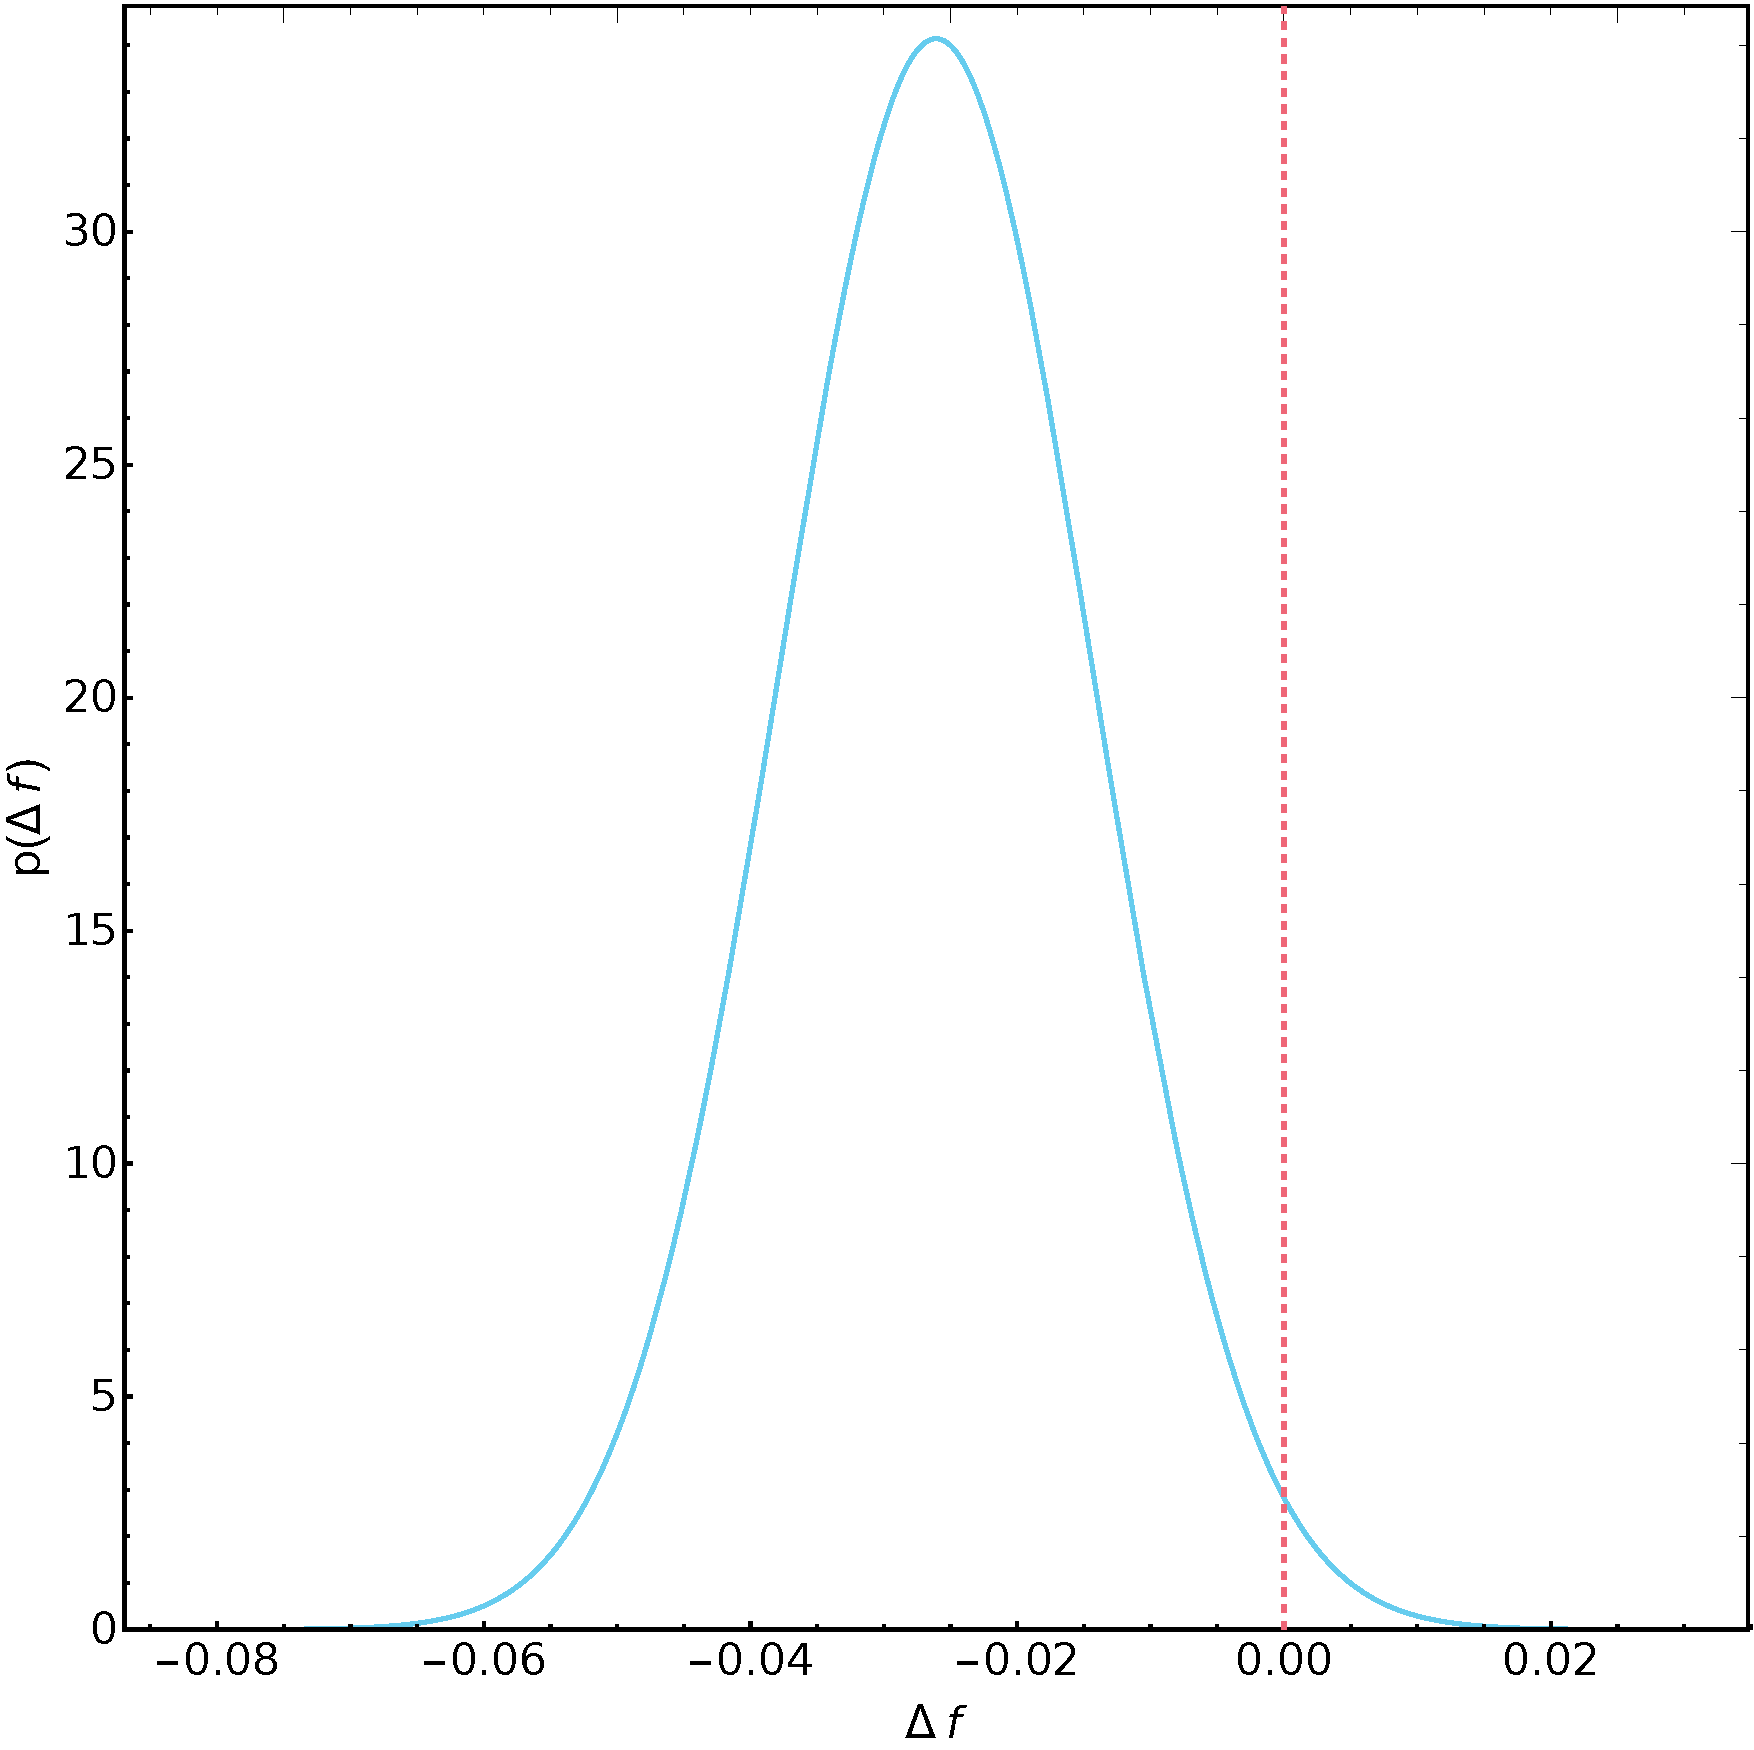
\includegraphics[width=0.49\linewidth]{example_diff.pdf}\hspace*{\stretch{1}}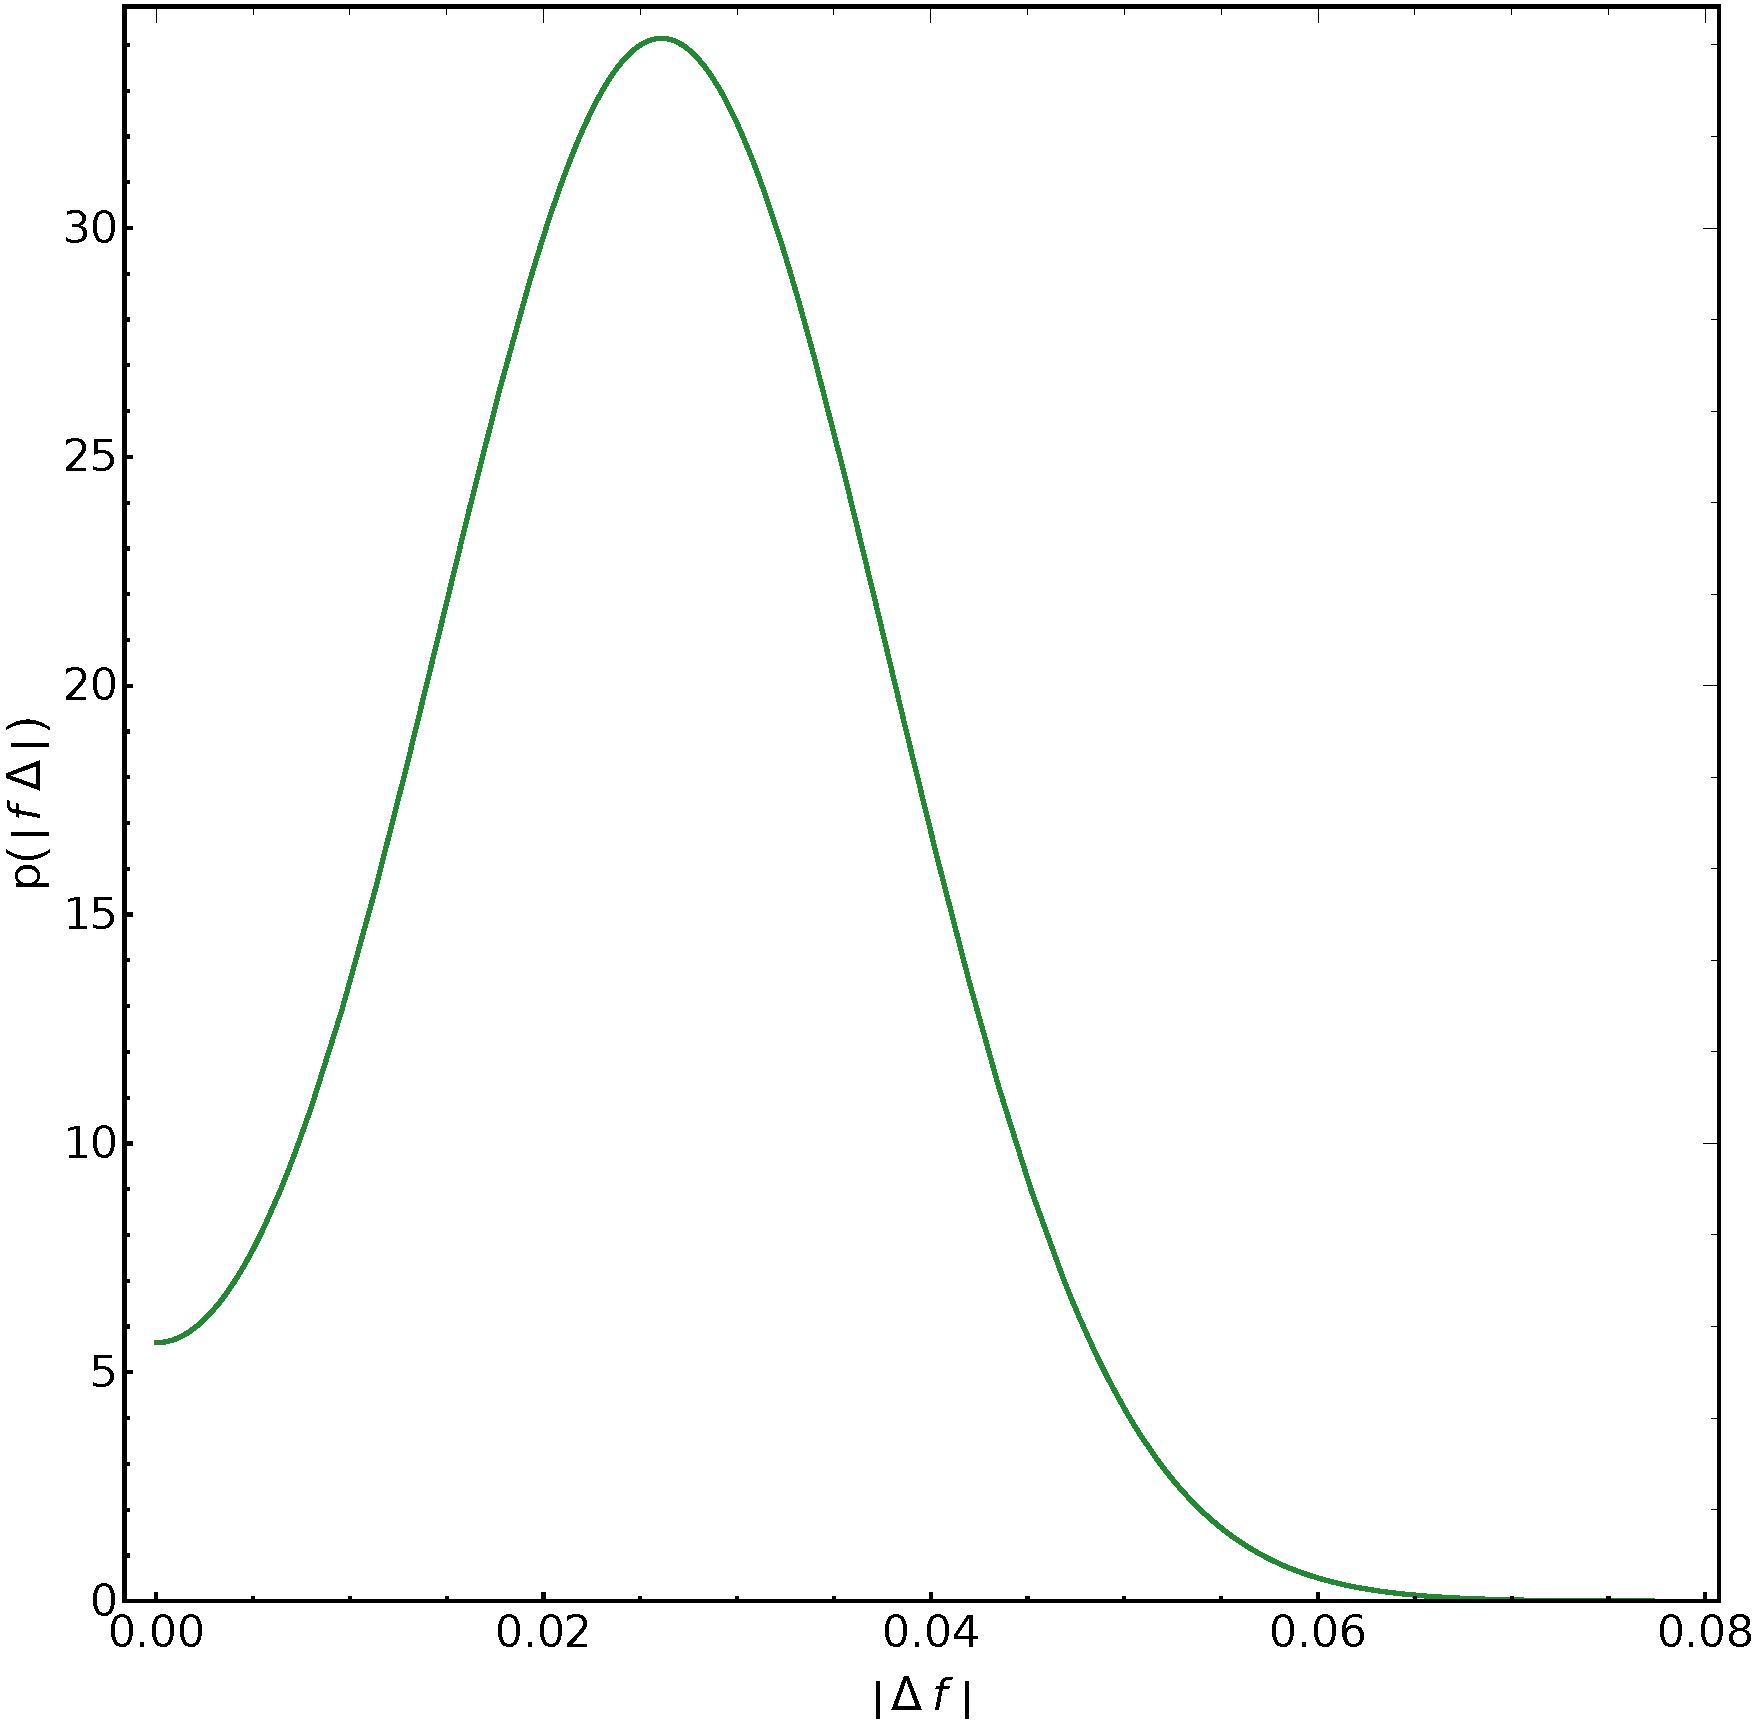
\includegraphics[width=0.49\linewidth]{example_absdiff.pdf}\\
 \caption{Example of uncertainty distributions about the
   conditional-frequency difference $\df$ and its absolute value
   $\abs{\df}$.}\label{fig:not-example_difference_distributions_old}
\end{figure}% scripts2/plot_curves.nb
% freq-1_1_conserv-spreads-sym_O-snp_6-spr_2.233.csv
% "spread_y",-2.23267970003192
% "EV_y",-0.0260880661493155
% "SD_y",0.0116846434125515
These distributions give us many pieces of information: for example, a
negative difference $\df$ is more plausible than a positive one; it is
8.3\% plausible that $\abs{\df}<0.01$, and therefore 91.7\% plausible that
$\abs{\df}>0.01$; it is 90\% plausible that $-0.045 < \df < -0.007$; and so
on. Several measures can be chosen to summarize the distribution with one
number. For example, we could use some minimal frequency difference we are
highly sure about, for example the lowest 10-quantile:
\begin{equation}\label{eq:not-significance_measure}
x\;\text{ such that }\; \pf(\abs{\df} > x)=0.9,
\end{equation}
or simply the expectation of the absolute value of the difference
\citep{leoneetal1961}:
\begin{equation}\label{eq:not-significance_measure_expabs}
\E\bigl(\abs{\df}\bigr) \equiv \sqrt{\frac{2}{\pu}}\sigma\exp\Biggl(-\frac{\mu^2}{2\sigma^2} \Biggr) + \mu \erf\Biggl( \frac{\mu}{\sqrt{2}\sigma} \Biggr),
\end{equation}
where $\mu$ and $\sigma$ are the mean and standard deviation of $\pf(\df)$.
For the plot of \fig~\ref{fig:example_difference_distributions} such
measures are $0.0112$ and $0.0262$.
% values obtained in scripts2/plot_curves.nb
\mynote{add maybe something about dependence of broadness on sample size, and
  \enquote{smoothing} as discussed by MacKay \amp\ Bauman Peto
  \citey[\sect~2.6]{mackayetal1995}.}

A more complete quantification of our uncertainty is the distribution
$\pf(f_{|\ya}, f_{|\yb})$ among the possible joint values of the two
conditional frequencies, from which $\pf(\df)$ can be calculated. This
joint distribution is also the optimal starting point when frequencies
conditional on allele combinations of several \snp\ are considered. Our
goal is therefore to quantify this joint \dob, given:
\begin{enumerate*}[label=(\arabic*)]
\item the conditional frequencies in a population sample, \item our initial
  information or guesses about such frequencies.
\end{enumerate*} In formulae, we want to assign a numerical value to
\begin{equation}\label{eq:not-p_goal}
  \pf(\ptext{conditional frequencies} \|
  \ptext{sample data}, \ptext{initial information}).
\end{equation}
In the rest of this section we shall calculate this \dob\ by methodically
applying the probability calculus.

\medskip

First let's observe that the approach just outlined is not dichotomous,
unlike a classical significance test. We are not asking whether the
frequency difference is \enquote{significant} or not. Rather, we find a
gradation of cases: from conditional frequencies likely to be very
distinct, to conditional frequencies likely to be very similar. These cases
can be sorted, for example with the measure of
formula~\eqref{eq:significance_measure}, obtaining a sequence of \snp s
with a decreasing belief of causal association with the symptom. How many
of these \snp s are to be selected for further study depends on one's
experimental and computational resources.
\textcolor{white}{If you find this you can claim a postcard from us.}


% In the next sections we use formula~\eqref{eq:intuitive_Bayes} to estimate
% the limit frequencies given a sample of $6029$ individuals from \mynote{***
%   details here}. We shall first focus on the conditional frequencies of
% each insomnia symptom given one \snp\ at a time. The inferences in this
% case are very simple, intuitive, and easily visualizable. In the subsequent
% sections we shall consider the study of each symptom given \emph{pairs} of
% \snp s, and the study of all possible eight \emph{symptom combinations}
% given one \snp\ at a time.



\subsection{Inference: concrete calculation}
\label{sec:not-inference}

Once we know the quantity we want to quantify our uncertainty about, the
calculation of our \dobs\ follows almost mechanically from the rules of the
probability calculus
\citep{jeffreys1939_r1983,cox1946,jaynes1994_r2003,hailperin1996}. This
calculus also shows which \dobs\ we must provide at the start, to arrive at
the desired ones.

The first step is to use Bayes's theorem:
\begin{multline}
  \label{eq:not-intuitive_Bayes}
  \pf(\ptext{frequencies} \| \ptext{data}, \ptext{initial info})
  \propto{}\\
  \pf(\ptext{data} \| \ptext{frequencies}, \ptext{initial info})
  \times
  \pf(\ptext{frequencies} \| \ptext{initial info}),
\end{multline}
which says that we need to provide two kinds of \dob: the plausibility of
obtaining our sampled data if we had known the conditional frequencies in
the larger population; and our initial guess about the conditional
frequencies, before we observed the data. The first is given by a simple
sampling formula. The second can be modelled in several reasonable ways;
we'll see, however, that they all lead to very similar conclusions about
the conditional frequencies and their difference, owing to the large size
of our sample. Let's give explicit expressions for both.

First of all, introduce some notation. The conditional frequencies are
denoted $f_{|\ya}$, $f_{|\yb}$ as above. The data $\yD$ consist in the
conditional frequencies observed in the sample: $F_{|\ya}$ is the fraction
showing the symptom among the sampled individuals having allele $\ya$, and
$F_{|\yb}$ is the analogous fraction for allele $\yb$. Finally, our initial
information $\yI$ consists in our initial beliefs and in the numbers
$N_{\ya}$, $N_{\yb}$ of sampled individuals having allele $\ya$ and $\yb$;
although these numbers are part of $\yI$ we will sometimes write them
explicitly besides $\yI$. (Note that $N_{\ya}$, $N_{\yb}$ are not part of
the \enquote{data} in the sense that they don't help us to update our
belief about the frequencies $f_{|\ya}$, $f_{|\yb}$ and therefore remain on
the right side of the conditional.)

\iffalse
In this section we do step by step the calculations outlined above. For
definiteness we consider onset insomnia ($\ysS$) and the \snp\ rs875994
with alleles $\ya$, $\yb$. The limit conditional frequencies are denoted
$f_{\ya}$ and $f_{\yb}$. The sample data, denoted by $\yD$,
consist of the number of individuals $F_{\ya}$ that show symptom
$\ysS$ among the sampled individuals having allele $\ya$, and the number
$F_{\yb}$ showing the same symptom among those having allele $\yb$.
Our initial information consists in the number $N_{\ya}$ of sampled
individuals with allele $\ya$, and the number $N_{\yb}$ with allele $\yb$.
The total number of sampled individuals is therefore $N_{\ya}+N_{\yb}$.
This initial information and our initial beliefs are denoted by $\yI$; the
numbers $N_{\ya}$, $N_{\yb}$ will often be indicated explicitly even though
they're part of $\yI$.
\fi

With this notation, Bayes's theorem above is written
\begin{multline}
  \labelbis{eq:intuitive_Bayes}
  \pf(f_{|\ya}, f_{|\yb} \| \yD, \yI)
  \propto
  \pf(\yD \|f_{|\ya}, f_{|\yb}, \yI)\;
  \pf(f_{|\ya}, f_{|\yb} \| \yI)
  \equiv{}\\
  \pf(F_{|\ya}, F_{|\yb} \|f_{|\ya}, f_{|\yb}, N_{\ya},N_{\yb},\yI)\;
  \pf(f_{|\ya}, f_{|\yb} \| N_{\ya},N_{\yb},\yI).
\end{multline}

\medskip

\subsection{Plausibility for the data given the frequencies}
\label{sec:not-p_data_from_freqs}

The plausibility of obtaining the data given the frequencies is given by
simple counting and symmetry. We have an arbitrarily large population where
a fraction $f_{|\ya}$ of individuals having allele $\ya$ show the symptom,
and a fraction $1- f_{|\ya}$ therefore don't show the symptom. We casually
observe $N_{\ya}$ individuals with allele $\ya$. The plausibility that a
fraction $F_{|\ya}$ of these show the symptom is then counted as a
\enquote{drawing with replacement} because of the arbitrarily large size of
the full population, given by a (rescaled) binomial distribution
\cites[\chap~3]{jaynes1994_r2003}[\sect~4.6]{ross1976_r2010}[\sect~VI.2]{feller1950_r1968}:
\begin{equation}
  \label{eq:not-sampling_belief}
  \pf( F_{|\ya} \| f_{|\ya},  N_{\ya}, \yI)
  =
\binom{N_{\ya}}{N_{\ya}\,F_{|\ya}}\;  {f_{|\ya}}^{N_{\ya}\,F_{|\ya}} \;
  {(1-f_{|\ya})}^{N_{\ya}\,(1-F_{|\ya})}.
\end{equation}

An analogous reasoning holds for allele $\yb$. Our belief about obtaining
the data is therefore
\begin{equation}
  \label{eq:not-sampling_belief_combined}
%  \pf(F_{|\ya},F_{|\yb} \|  f_{|\ya},f_{|\yb}, N_{\ya}, N_{\yb}, \yI)
  \pf(\yD \|  f_{|\ya},f_{|\yb}, \yI)
  =
 \prod_{x=\ya,\yb} \binom{N_{x}}{N_{x}\,F_{|x}}\;{f_{|x}}^{N_{x}\,F_{|x}} \;
  {(1-f_{|x})}^{N_{x}\,(1-F_{|x})}.
\end{equation}





\subsection{Plausibilities for the frequency differences}
\label{sec:not-p_df}

We finally find an approximate expression for our final \dob\ about the
conditional-frequency difference $\df$. The density is also approximately
normal, and for each initial state of knowledge $\yI=\yIu,\yIc$ its mean
and variance can be found by the standard formulae \mynote{give ref for
  these}
\begin{align}
  \label{eq:not-mean_final_diff}
    &\E(f_{|\ya}- f_{|\yb} \| \yD, \yI) =
    \E(f_{|\ya} \| \yD, \yI) -
    \E( f_{|\yb} \| \yD, \yI),
    % \frac{N_{\ya}\,F_{|\ya}+1}{N_{\ya}+2} -
    % \frac{N_{\yb}\,F_{|\yb}+1}{N_{\yb}+2}  
    \\[\jot]
  \label{eq:not-cov_final_diff}
    &\var(f_{|\ya}- f_{|\yb} \| \yD, \yI) =
      \var(f_{|\ya} \| \yD, \yI) +
      \var(f_{|\yb} \| \yD, \yI) -
      2\cov(f_{|\ya},f_{|\yb} \| \yD, \yI),
      % \frac{(N_{\ya}F_{|\ya}+1)\,[N_{\ya}\,(1-F_{|\ya})+1)}{(N_{\ya}+2)^2\,(N_{\ya}+3)}
      % +
      % \frac{(N_{\yb}F_{|\yb}+1)\,[N_{\yb}\,(1-F_{|\yb})+1)}{(N_{\yb}+2)^2\,(N_{\yb}+3)}
\end{align}
from the formulae~\eqref{eq:stats_final_unif},
\eqref{eq:stats_final_conserv} given in the previous section.







% Combining \eqns~\eqref{eq:formal_hierarchic_approx},
% \eqref{eq:def_ff_given_Aq}, \eqref{eq:def_beta} we thus arrive at the
% following explicit approximate formula for our belief about the conditional
% frequencies given the data:
% \begin{multline}
%   \label{eq:not-formal_hierarchic_approx_final}
%   \pf(f_{|\ya}, f_{\yb} \| \yD, \yI) \approx
%   \dbeta(f_{|\ya} \| \yuam,\yubm)\;
%   \dbeta(f_{\yb} \| \yuam,\yubm)\\
%   \text{with
%     $(\yuam,\yubm)$ maximizing~\eqref{eq:to_optimize}}.
% \end{multline}
%  \mynote{ref here to \citep{mackay1996}}






\begin{figure}[b!]%{r}{0.4\linewidth} % with wrapfigure
 \centering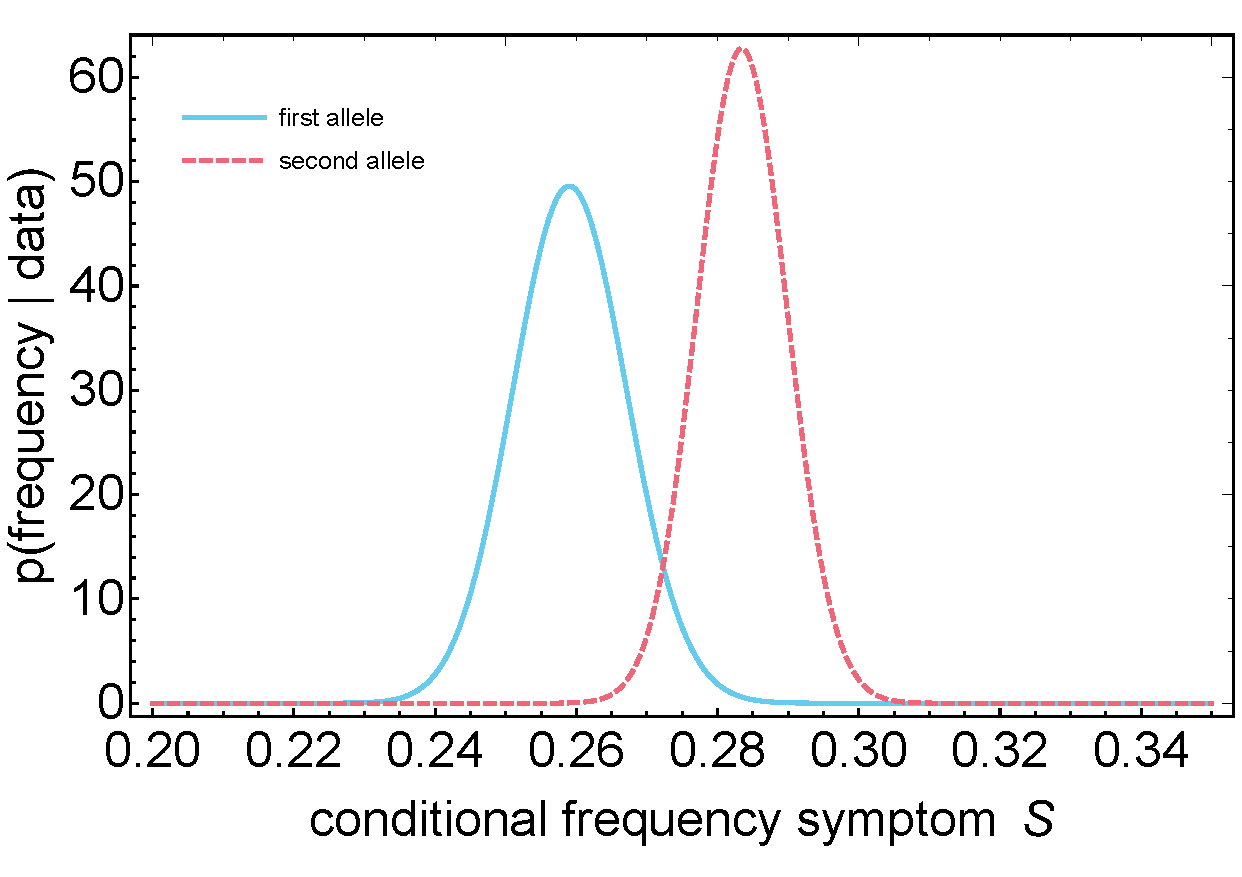
\includegraphics[width=0.75\linewidth]{example_distr_condfreqs.pdf}\\
\caption{Example of distributions of belief}\label{fig:not-example_distributions}
\end{figure}% scripts/single_gene_condfreqs_thetamax.nb
%% EVs: 0.25917, 0.283506; SDs: 0.00804727, 0.00635616
%% overlap at 0.01 = 0.0321908



\begin{figure}[b!]%{r}{0.4\linewidth} % with wrapfigure
 \centering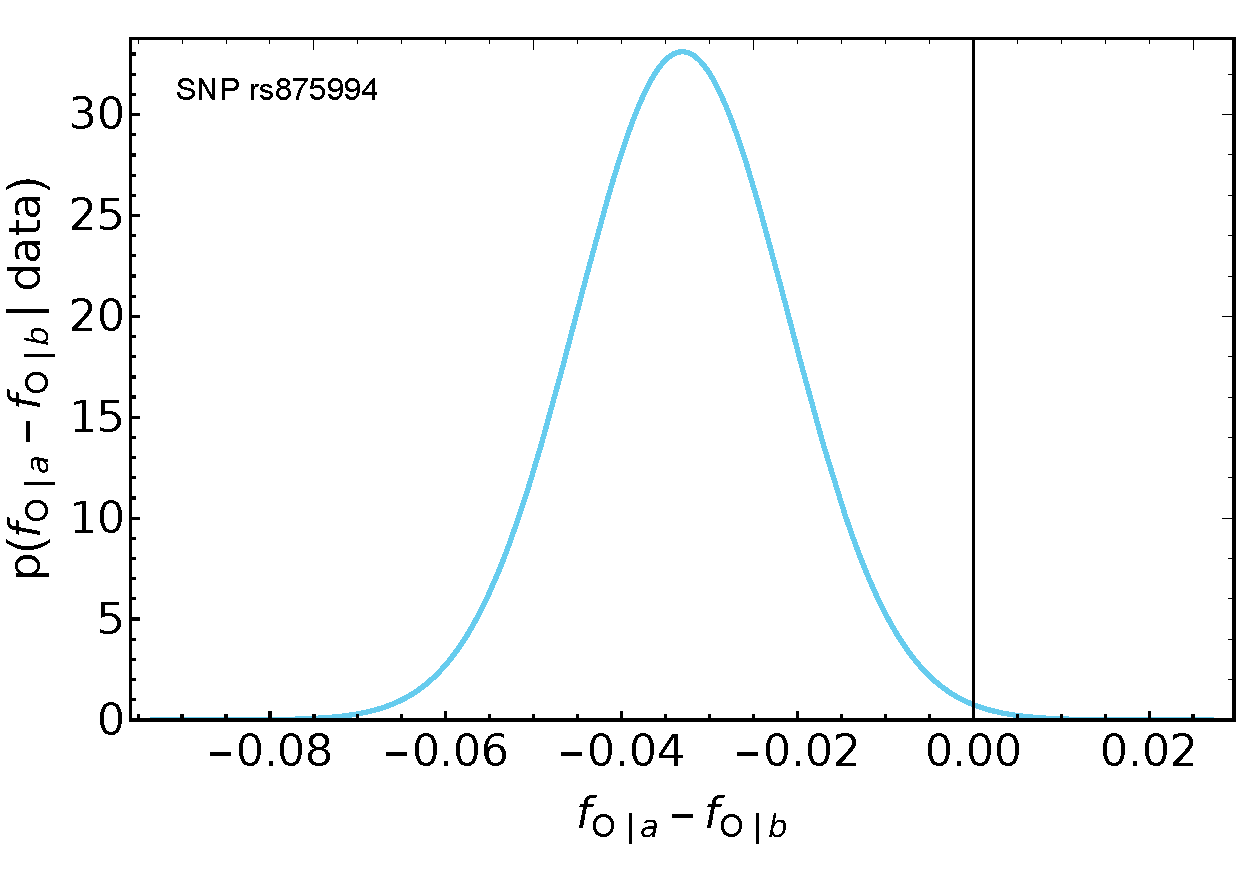
\includegraphics[width=0.75\linewidth]{difference_symA_snp6.pdf}\\
 \caption{Distribution for the difference between the frequencies
   $f_{\ysO\|\ya}$, $f_{\ysO\|\yb}$ of onset insomnia ($\ysO$) conditional on
   the two alleles of \snp\ rs875994}\label{fig:not-difference_distributions}
\end{figure}% scripts/condfreqs_general_tests.nb
%% snp #6,
%% EV: -0.0330998, SD: 0.0120472
%% EV/SD: 2.75
%% 0.0274176 within 0.01

\newpage
%\renewcommand*{\appendixpagename}{Appendix}
%\renewcommand*{\appendixname}{Appendix}
%\appendixpage
%\appendix


The uniform state of knowledge is given by the simple density
\begin{equation}
  \label{eq:not-uniform_prior}
  \pf(f_{|\ya}, f_{|\yb} \| \yIu)%\;\di f_{|\ya}\,\di f_{|\yb}
  =1.%\di f_{|\ya}\,\di f_{|\yb}.
\end{equation}
The conservative state of knowledge is given by the following integral:
\begin{subequations}
  \label{eq:not-conservative_prior}
  \begin{gather}
    \pf(f_{|\ya}, f_{|\yb} \| \yIc)%\;\di f_{|\ya}\,\di f_{|\yb}
    =
    \int_{\mathrlap{0}}^{\mathrlap{\infty}}\di\yua
    \int_{\mathrlap{0}}^{\mathrlap{\infty}}\di\yub\;
    \pf(f_{|\ya}, f_{|\yb} \| \yua,\yub,\yIc)\;
    \pf(\yua,\yub \| \yIc)%\;\di f_{|\ya}\,\di f_{|\yb}
    \\
    \shortintertext{with}
    \label{eq:not-beta_product}
    \pf(f_{|\ya}, f_{|\yb} \| \yua,\yub,\yIc)\defd
    \dbeta(f_{|\ya} \| \yua,\yub)\;
    \dbeta(f_{|\yb} \| \yua,\yub),
    \\
    \label{eq:not-p_initial_parameters}
    \pf(\yua,\yub \| \yIc)\defd \frac{1}{u+v}\,\dgamma(u+v \| 1, 1000)
  \end{gather}
  where $\dbeta$ and $\dgamma$ are beta and gamma densities:
  \begin{gather}
    \label{eq:not-def_beta}
    \dbeta(f \| \yua,\yub) \defd
    \frac{\Gamma(\yua+\yub)}{\Gamma(\yua)\,\Gamma(\yub)}\;
    f^{\yua-1}\;(1-f)^{\yub-1},
    \qquad  \yua,\yub>0,
    \\
    \label{eq:not-def_gamma}
    \dgamma(\yA \| 1, 1000) \defd
    \frac{1}{1000}\,\exp(-\yA/1000).
  \end{gather}
\end{subequations}
The integral expression~\eqref{eq:conservative_prior} can be interpreted as
follows: we consider several independent beliefs about the two frequencies
-- the product of beta densities, depending on identical shape parameters
-- and then weigh and mix them together to arrive at a belief that is not
independent about the two frequencies. This also corresponds to defining a
so-called hierarchic model \citep{good1980}. The particular shape and scale
values of the gamma density are chosen so as to concentrate our initial
belief along the $(f_{|\ya}, f_{|\yb})$ diagonal. The use of beta densities
in this problem seems to have been first endorsed by G. F. Hardy
\citey{hardy1889}; Good \citey[\sect~4.1]{good1965}[\sect~4]{good1980}
motivates the use of their mixtures. We discuss further interpretations of
this initial state of knowledge in appendix***.





\section{Generalizations}

\subsection{Generalization to \snp\ combinations}
\label{sec:not-generalize_snp}

The ideas and mathematical results discussed in the Method section are
easily generalized to the frequencies of a symptom conditional on the
combination of the alleles of two or more \snp s. Consider the simplest
case of two; denote the two alleles of the first \snp\ by $\ya$, $\yb$, and
of the second $\yas$, $\ybs$. We then have $2^2$ conditional frequencies
$f_{|\ya\yas}$, $f_{|\ya\ybs}$, $f_{|\yb\yas}$, $f_{|\yb\ybs}$ and we want
to quantify the plausibility density
$\pf(f_{|\ya\yas},f_{|\ya\ybs},f_{|\yb\yas},f_{|\yb\ybs} \| \yD, \yI)$
given the conditional frequencies $F_{|\ya\yas}$, $F_{|\ya\ybs}$,
$F_{|\yb\yas}$, $F_{|\yb\ybs}$ observed in a sample of size
$N_{\ya\yas}+N_{\ya\ybs}+N_{\yb\yas}+N_{\yb\ybs}$.

Bayes's theorem~\eqref{eq:intuitive_Bayes} applies as before. The sampling
plausibility~\eqref{eq:sampling_belief_combined}, obtained by the same
reasoning, generalizes to the product over
$x=\ya\yas,\ya\ybs,\yb\yas,\yb\ybs$. The uniform initial state of knowledge
has still unit density as in~\eqref{eq:uniform_prior}. The conservative
initial state of knowledge~\eqref{eq:conservative_prior} generalizes to the
mixture of the product of $2^2$ beta distributions, one for each
combination of alleles, conditional on the same parameters $\yua$, $\yub$.
The rest of the calculations proceed analogously.

In this case we have $\tbinom{4}{2}\equiv 6$ conditional-frequency
differences of interest: $f_{|\ya\yas}- f_{|\ya\ybs}$,
$f_{|\ya\yas}- f_{|\yb\yas}$, $f_{|\ya\yas}- f_{|\yb\ybs}$, and so on. The
analysis of the results therefore offers more interesting possibilities.

\subsection{Generalization to symptom combinations}
\label{sec:not-generalize_symptoms}

The Method section is also easily generalized to the conditional
frequencies of non-dichotomous symptoms, or of symptom combinations. For
example, for our study we could consider the $2^3$ combinations: individual
with no symptoms, or with only symptom $\ysO$ present, or with only
symptoms $\ysO$ and $\ysM$ present, and so on up to all three symptoms
$\ysO$, $\ysM$, $\ysT$ present. We can denote these cases by $\ysO$,
$\ysO$, $\ysO\ysM$, and so on. Each of these frequencies would be
conditional on whether the individual has allele $\ya$ or $\yb$ of a
particular \snp. We thus have two conditional-frequency distributions:
\begin{equation}
  \label{eq:not-f_distr_symptom_combo}
  \begin{aligned}
    &(f_{\ysO\|\ya},f_{\ysO\|\ya},\dotsc,f_{\ysO\ysM\|\ya},\dotsc,f_{\ysO\ysM\ysT\|\ya}),
    \qquad&\sum_{y} f_{y\|\ya} =1,
      \\
    &(f_{\ysO\|\yb},f_{\ysO\|\yb},\dotsc,f_{\ysO\ysM\|\yb},\dotsc,f_{\ysO\ysM\ysT\|\yb}),
    \qquad&\sum_{y} f_{y\|\yb} =1.
  \end{aligned}
\end{equation}



\subsection{Choices of initial beliefs and meaning of the parameters}
\label{sec:not-choices_prior_info}


The parameters $\yu$ of the Dirichlet density for the frequency
distribution $\yf$ have very intuitive meanings, even more evident if we
rewrite them as their sum and a pair of normalized parameters:
\begin{equation}
  \label{eq:not-rewrite_params}
  \yA \defd \ysum\yu,
  \qquad
  \yq\defd\yu/\sum\yu.
\end{equation}
The normalized parameters $\yq$ are the expected frequency distribution:
\begin{equation}
  \label{eq:not-meaning_normalized_parameters}
  \E(\yf \| \yu) = \yq
\end{equation}
The sum of the parameters $\yA$ expresses the sharpness of the
distribution, as seen from the covariance matrix:
\begin{equation}
  \label{eq:not-variances_covariances}
  \var(f_i \| \yu) = \frac{\yqq_i\;(1-\yqq_i)}{\yA+1},
  \qquad
  \cov(f_i\,f_j \| \yu) = -\frac{\yqq_i\,\yqq_j}{\yA+1}.
\end{equation}
In fact, from the update formula*** we see that $\yA$ quantifies the amount
of data necessary to modify our initial belief.



\[
  \frac{  \E(f_{\ysO\|\ya} - f_{\ysO\|\yb} \| \yD, \yI)}{
    \std(f_{\ysO\|\ya} - f_{\ysO\|\yb} \| \yD, \yI)}
\]

*********************************

This construction has the interesting consequence for our updated belief
$\pf(f_{|\ya}, f_{\yb} \| \yD, \yI)$. According to Bayes's
theorem~\eqref{eq:intuitive_Bayes} combined with our initial
belief~\eqref{eq:beta_gamma_prior} it is given by
\begin{equation}
  \label{eq:not-straight_Bayes}
  \pf(f_{|\ya}, f_{\yb} \| \yD, \yI)
  \propto
  \pf(\yD \| f_{|\ya}, f_{\yb} \| \yI)\;
  \pf(f_{|\ya}, f_{\yb} \| \yI),
\end{equation}
but, as shown in appendix~\ref{sec:bayes_hierarcic}, it can also be written
in the following way:
\begin{equation}
  \label{eq:not-formal_hierarchic}
  \pf(f_{|\ya}, f_{\yb} \| \yD, \yI) =
  \tint\di\yua\tint\di\yub\;
  \pf(f_{|\ya}, f_{\yb}\| \yD,\yua,\yub,\yI)\;
  %   \dbeta(f_{|\ya} \| \yua,\yub)\,
  % \dbeta(f_{\yb} \| \yua,\yub)\;
  \dA(\yua,\yub \|\yD, \yI),
\end{equation}
with the normalized density $\dA(\yua,\yub \|\yD, \yI)$ defined by
\begin{multline}
  \label{eq:not-update_hyperparameter}
  \dA(\yua,\yub \|\yD, \yI) \propto   \dA(\yua,\yub \|\yI)
\times{}\\
%\Bigl[
\underbrace{\tint\di f_{|\ya}\tint\di f_{\yb}\;
  \pf(\yD \|f_{|\ya}, f_{\yb}, \yI)\;
 \pf(f_{|\ya}, f_{\yb} \|\yua,\yub, \yI)}_{\zerob{\footnotesize${}\defs\pf(\yD \|\yua,\yub,\yI)$}}.
      % \dbeta(f_{|\ya} \| \yua,\yub)\,
      % \dbeta(f_{\yb} \| \yua,\yub)
%       \Bigr]
\end{multline}
It is as if $\yua$, $\yub$ were unknown parameters with initial belief
density $\dA(\yua,\yub \|\yI)$, and our update for the frequencies proceeded by
first updating our belief about the parameters,
\eqn~\eqref{eq:update_hyperparameter}, and then marginalizing them out,
\eqn~\eqref{eq:formal_hierarchic}. This is a so-called \emph{hierarchic}
model \citep{good1980}. This hierarchic way of thinking often helps in
constructing densities that better represent our initial beliefs, and also
leads to formulae that can be better approximated when exact computation is
unfeasible. A point rarely emphasized in the literature, though, is that
there is no mathematical difference between a hierarchic and a
non-hierarchic model: we could forget about the integrals in
formula~\eqref{eq:beta_gamma_prior} and about the update
formula~\eqref{eq:formal_hierarchic}, and simply treat
$\pf(f_{|\ya}, f_{\yb} \| \yI)$ as the density depicted in
\fig~\ref{fig:initial_belief}, with update~\eqref{eq:intuitive_Bayes}. The
results would be the same. Further discussion about the formulae above is
given in \sect***.


With large sample sizes the density $\dA(\yua,\yub \|\yD, \yI)$ turns out to
be so peaked with respect to
$\pf(f_{|\ya}, f_{\yb}\| \yua,\yub,\yI)$ that it can be considered
as a Dirac delta centred on the parameters $\yuam$, $\yubm$ that maximize it.
We thus obtain a good approximation of the updated
belief~\eqref{eq:formal_hierarchic} that doesn't involve parameter integration:
\begin{multline}
  \label{eq:not-formal_hierarchic_approx}
  \pf(f_{|\ya}, f_{\yb} \| \yD, \yI) \approx
  \pf(f_{|\ya}, f_{\yb}\| \yuam,\yubm,\yI)\\
  \text{with}\quad
  (\yuam,\yubm) \defd \argmax_{\yua,\yub}\dA(\yua,\yub \|\yD, \yI).
\end{multline}
The maximum of $\dA(\yua,\yub \|\yD, \yI)$, or better of its logarithm, can
easily be found with most optimization methods. The explicit expression to
be optimized, discussed in appendix***,
\begin{equation}
  \label{eq:not-to_optimize}
  \yna\,[\ln\Gamma(\tsum_s\yu_s) - \tsum_s\ln\Gamma(\yu_s)]
  -\sum_{\mathclap{x=\ya,\yb}}
  [\ln\Gamma(N_x+\tsum_s\yu_s) - \tsum_s\ln\Gamma(N_xF_{s\|x}+\yu_s)]
\end{equation}


\section{Derivation of Bayes's theorem in hierarchic form}
\label{sec:not-bayes_hierarcic}

We write Bayes's theorem~\eqref{eq:straight_Bayes} with our initial
belief~\eqref{eq:beta_gamma_prior} written in full:
\begin{equation}
  \label{eq:not-straight_Bayes_full_prior}
  \pf(f_{\ysO\|\ya}, f_{\ysO\|\yb} \| \yD, \yI)
  \propto
  \tint\di\yA\tint\di\yq\;
    \pf(\yD \| f_{\ysO\|\ya}, f_{\ysO\|\yb} \| \yI)\;
 \pf(f_{\ysO\|\ya}, f_{\ysO\|\yb} \|\yA,\yq, \yI)\;
  \dA(\yA,\yq \|\yI).
\end{equation}
Multiplying and dividing within the integral with the expression
\begin{equation}
  \label{eq:not-def_Aq_given_data}
    \pf(\yD \|\yA,\yq,\yI)\defd
\tint\di f_{\ysO\|\ya}\tint\di f_{\ysO\|\yb}\;
  \pf(\yD \|f_{\ysO\|\ya}, f_{\ysO\|\yb}, \yI)\;
  \pf(f_{\ysO\|\ya}, f_{\ysO\|\yb}\| \yA,\yq,\yI)
      % \dbeta(f_{\ysO\|\ya} \| \yA,\yq)\,
      % \dbeta(f_{\ysO\|\yb} \| \yA,\yq)
\end{equation}
we obtain the alternative form~\eqref{eq:formal_hierarchic}



Combining together the sampling
formula~\eqref{eq:sampling_belief_combined}, the expression of the beta
density~\eqref{eq:def_beta}, and the update
formula~\eqref{eq:update_hyperparameter} we obtain
\begin{multline}
  \label{eq:not-parameter_posterior_first}
  \dA(\yA,\yq \|\yD, \yI) \propto
    \dA(\yA,\yq) \times{}\\
  \Bigl[   \tint\di f_{\ysO\|\ya}\tint\di f_{\ysO\|\yb}\;
  \dbeta\Bigl(f_{\ysO\|\ya} \|[\Big] \yA+N_{\ya},
  \frac{\yA\yq+N_{\ya}F_{\ysO\|\ya}}{\yA+N_{\ya}}
    \Bigl)\;
  \dbeta\Bigl(f_{\ysO\|\yb} \|[\Big] \yA+N_{\yb},
  \frac{\yA\yq+N_{\yb}F_{\ysO\|\yb}}{\yA+N_{\yb}}
    \Bigr)
       \Bigr]
%  \pf(f_{\ysO\|\ya}, f_{\ysO\|\yb} \|\yA,\yq, \yI)\;
\end{multline}


\section{Summary of the main formulae}

We have a sample of size $n$. We check the subsample of individuals that
have a particular allele, say Bx, for a particular gene, say rs697680\_A.
Suppose that in this subsample $n_0$ individuals \emph{don't} show symptom
A and $n_1$ \emph{do} show symptom A. This also means that the size of our
subsample (individuals with allele Bx) is $n \defd n_0+n_1$.

Our \dob\ about the frequency $f_1$ of symptom A among the individuals with
allele Bx in an \emph{infinite} population is a Beta distribution with
parameters $n_0+\theta_0$, $n_1+\theta_1$, with
$\theta \defd \theta_0+\theta_1$:
\begin{multline}
  \label{eq:not-beta_fr}
  \pf(f_1 \| n_0,n_1,\theta_0,\theta_1)\;\di f_1 ={}\\
  \frac{\Gamma(n+\theta)}{\Gamma(n_0+\theta_0)\;\Gamma(n_1+\theta_1)}
  \; (1-f_1)^{n_0+\theta_0-1}\;{f_1}^{n_1+\theta_1-1} \;\di f_1
\end{multline}
This distribution has expected value and variance
\begin{equation}
  \label{eq:not-exp_value}
  \begin{split}
  \E(f_1 \| n_0, n_1, \theta_0,\theta_1) &= \frac{n_1+\theta_1}{n+\theta},
  \\
  \var(f_1 \|  n_0, n_1, \theta_0,\theta_1) &=
  \frac{(n_0+\theta_0)\;(n_1+\theta_1)}{(n+\theta)^2\;(n+\theta+1)}.
\end{split}
\end{equation}



\mynote{Possible further developments: use of hyper-Dirichlet priors, use
  of graphical models to infer causal relationships
  \citep{pearl2000_r2009}}

\[
\begin{aligned}
\pf(f \|\yD)  &\propto \pf(\yD \| f)\;\pf(f \| \yI)
  \\
  &\propto \pf(\yD \| f)\;\int\di u\, \pf(f \|u)\, \pf(u\| \yI)
  \\
  &\propto \int\di u\,\pf(\yD \| f)\; \pf(f \|u)\; \pf(u\| \yI)
  \\
  &\propto \int\di u\,\pf(\yD \| f,u)\, \pf(f \|u)\;
    \pf(\yD \| u)\, \pf(u\| \yI)
  \\
  &\propto \int\di u\,\pf(f \| D,u)\;
    \pf(u \| \yD)
\end{aligned}
\]

\[
  \begin{aligned}
    \pf(u \|\yD)
    &\propto \int\di f\, \pf(\yD \| f)\,\pf(f \| u)\;\pf(u \| \yI)
    \\
    &\propto
      \prod_{x=\ya,\yb}\Biggl[ 
      \frac{\Gamma(\tsum_su_s)}
      {\tprod_s\Gamma(u_s)}\;
      \frac{\tprod_s\Gamma(N_xF_{s\|x}+u_s)}
      {\Gamma(N_x+\tsum_su_s)}
       \Biggr]
  \end{aligned}
\]


\[
  \pf(f_{\ysO\|\ya}, f_{\ysO\|\yb} \| \yD, \yI) \approx
  \pf(f_{\ysO\|\ya}, f_{\ysO\|\yb}\| \yuam,\yubm,\yI)
\]


%%% Local Variables: 
%%% mode: LaTeX
%%% TeX-PDF-mode: t
%%% TeX-master: t
%%% End: 
